\documentclass[11pt,a4paper]{article}

\usepackage[utf8]{inputenc}
\usepackage[margin=1in]{geometry}
\usepackage{amsmath,amssymb,amsfonts}
\usepackage{graphicx}
\usepackage{booktabs}
\usepackage{cite}
\usepackage{hyperref}
\usepackage{lineno}
\usepackage{caption}
\usepackage{microtype}
\usepackage{xcolor}
\usepackage{authblk}

\hypersetup{
    colorlinks=true,
    linkcolor=blue!70!black,
    citecolor=blue!70!black,
    urlcolor=blue!70!black
}

\title{\textbf{Decoupling Total Barometric Pressure from Oxygen Partial Pressure in the \textit{Arabidopsis thaliana} Spaceflight Exploration Atmosphere Using the TabPFN v2 Tabular Foundation Model: Molecular Hubs, Single-Nucleus Trajectories, and Physiological Rescue}}

\author[1,*]{Richard J. Barker}
\author[1]{Anna-Lisa Paul}
\author[1]{Robert J. Ferl}
\affil[1]{Interdisciplinary Center for Biotechnology Research and Department of Horticultural Sciences, University of Florida, Gainesville, FL 32611, USA}
\affil[*]{Corresponding author: \texttt{dr-richard-barker@ufl.edu}}

\date{\today}

\begin{document}

\maketitle

\begin{abstract}
Future crewed lunar and Martian surface habitats, extravehicular activity (EVA) staging airlocks, and bioregenerative life-support systems will operate under NASA's reduced-pressure, oxygen-enriched \textbf{Exploration Atmosphere} ($56.54\text{ kPa}$ [$8.2\text{ psia}$], $34\%\ \text{O}_2$, oxygen partial pressure $p\text{O}_2 = 19.22\text{ kPa}$; pre-EVA staged decompression $70.33\text{ kPa}$ [$10.2\text{ psia}$], $26.5\%\ \text{O}_2$, $p\text{O}_2 = 18.64\text{ kPa}$). While enriching fractional $\text{O}_2$ restores normoxic $p\text{O}_2$, reducing total barometric pressure ($P_{\text{total}}$) inversely accelerates binary gas and water-vapor diffusivity ($D \propto P_{\text{total}}^{-1}$; $1.72\times$ faster at $56.54\text{ kPa}$ than at $97\text{ kPa}$ ISS cabin pressure), thinning the boundary layer and accelerating transpiration independently of cellular oxygen availability. However, small sample sizes ($n = 9\text{--}130$ per study), high feature dimensionality ($p = 22,746$ probesets), and historical metadata ambiguities have prevented classical machine learning models from cleanly separating pure barosensory ($P_{\text{total}}$) signaling from hypoxia ($p\text{O}_2$) signaling or linking these molecular hubs to cell-type trajectories and whole-plant physiology. Here, we harmonize a 12-dataset multi-omics compendium spanning 281 microarray hybridizations, 40,860 single-nucleus root-tip transcriptomes, 326 physiological gas-exchange and chlorophyll fluorescence records, LC-MS metabolomics across factorial pressure $\times$ humidity regimes, and 5,454 iTRAQ submergence proteins, and apply the \textbf{TabPFN v2} prior-data fitted tabular foundation model to resolve the plant response to exploration atmospheres. A forensic audit ledger tracking all 148 series-level GSM records deduplicates 18 shared arrays to establish 130 unique hypobaric arrays passing standard Affymetrix array QC (NUSE medians $1.00 \pm 0.25$, RLE IQRs $0.79 \pm 0.37$, percent present $81.7 \pm 10.0\%$), and resolves disputed $75\text{ kPa}$ arrays as Shoots ($P(\text{Shoot}\mid\mathbf{x}) > 0.99$). Under leak-free condition-grouped cross-validation, TabPFN v2 outperforms classical baselines across continuous Hypobaria Index regression ($R^2 = 0.9134$), Hypoxia Index regression ($R^2 = 0.9733$), and 4-class regime classification ($\text{ROC\_AUC} = 0.9623$, Accuracy = $86.21\%$). Orthogonal partial regression with empirical Bayes variance moderation reveals 1,003 Pure Hypoxia hubs, 380 Pure Barosensory hubs, and 21 Additive Dual Hubs. Single-nucleus transcriptomics and cell-type translatomes show strict spatial partitioning between epidermal barosensing and pan-lineage hypoxia. Physiological and metabolomic triangulation at $62\text{ kPa}$ reveals that boundary-layer vapor stripping elevates evaporative demand by $+73.23\%$ and halves net carbon assimilation, while elevating relative humidity to $70\%\ \text{RH}$ rescues chloroplast oxylipin galactolipids. Finally, Leave-One-Condition-Out validation and counterfactual synthesis indicate that while $34\%\ \text{O}_2$ enrichment mitigates $>88\%$ of root anaerobic activation, physical barosensory remodeling persists—establishing that humidity/VPD compensation ($75\text{--}80\%\ \text{RH}$) provides an immediate, non-genetic engineering countermeasure for lunar and Martian habitation.
\end{abstract}

\section*{Introduction}
Long-duration crewed space exploration requires transitioning from the International Space Station (ISS) cabin atmosphere ($97\text{--}101.3\text{ kPa}$, $21\%\ \text{O}_2$, $p\text{O}_2 \approx 20.37\text{--}21.27\text{ kPa}$) to reduced-pressure, oxygen-enriched habitats designed to minimize structural hull mass, gas leakage, and pre-extravehicular activity (EVA) nitrogen denitrogenation time \cite{norcross2013effects, paul2006spaceflight, zhou2017dissecting}. Specifically, NASA's Exploration Atmosphere architecture established a primary lunar/Martian habitat setpoint of $56.54\text{ kPa}$ ($8.2\text{ psia}$) at $34\%\ \text{O}_2$ ($p\text{O}_2 = 19.22\text{ kPa}$) and a staged pre-EVA decompression setpoint of $70.33\text{ kPa}$ ($10.2\text{ psia}$) at $26.5\%\ \text{O}_2$ ($p\text{O}_2 = 18.64\text{ kPa}$) \cite{norcross2013effects}. While raising fractional oxygen concentration ($F_{\text{I}}\text{O}_2$) maintains near-normoxic alveolar $p\text{O}_2$ for astronaut crews, reduced total barometric pressure ($P_{\text{total}}$) introduces a fundamental thermodynamic physical consequence for plants.

By Chapman--Enskog kinetic gas theory, binary molecular diffusivity $D_{ij}$ scales inversely with total pressure:
\begin{equation}
D_{ij}(P_{\text{total}}, T) = D_{ij}(P_0, T) \cdot \left(\frac{P_0}{P_{\text{total}}}\right)
\end{equation}
Consequently, reducing total pressure from $97\text{ kPa}$ to $56.54\text{ kPa}$ increases gas-phase molecular diffusivity by $D/D_0 = 1.72\times$ (and by $1.94\times$ at $50\text{ kPa}$ and $3.88\times$ at $25\text{ kPa}$), thinning the leaf boundary layer and accelerating transpiration \cite{corey2002gaseous, richards2006growth, paul2004hypobaric, paul2017spaceflight, lucia2025physiological}. When plants encounter uncompensated hypobaric air, they experience compound stress combining cellular hypoxia ($p\text{O}_2 = 5.25\text{--}15.75\text{ kPa}$, stabilizing group VII ETHYLENE RESPONSE FACTOR [ERF-VII] factors via PLANT CYSTEINE OXIDASE [PCO] inhibition \cite{gibbs2011homeostatic, licausi2011oxygen, mustroph2009profiling}) with physical barosensory stress ($D \propto P_{\text{total}}^{-1}$ boundary-layer acceleration and cell-wall mechanical strain \cite{zhou2017dissecting}). Historical studies observed substantial anaerobic induction, fostering the perception that hypobaria is predominantly hypoxic.

Here, we leverage the \textbf{TabPFN v2} tabular foundation model \cite{hollmann2025accurate} and the \textbf{Plant PhysioSpace} stress autodecoder \cite{esfahani2021plant} across a harmonized 12-dataset multi-omics compendium to resolve the plant response to spaceflight exploration atmospheres. We forensically audit the hypobaric microarray compendium, decouple $P_{\text{total}}$ from $p\text{O}_2$, map molecular hubs across 19 cell-type translatomes and 40,860 single nuclei, connect hubs to whole-plant gas exchange and metabolomics, and synthesize counterfactual predictions at NASA Exploration Atmosphere setpoints.

\section*{Results}

\subsection*{Workpackage 1: Forensic Metadata Audit and Probabilistic Organ Resolution}
A systematic audit of the four core hypobaric Affymetrix ATH1 microarray series (\texttt{GSE87867}, \texttt{GSE87868}/\texttt{OSD-136}, \texttt{GSE87903}, and \texttt{GSE87904}; 148 series-level records across 22,746 biological probesets) revealed that 18 GSM accessions (\texttt{GSM2342073}--\texttt{GSM2342090}) were dual-listed in both \texttt{GSE87867} and \texttt{GSE87903}. Pairwise correlation confirmed exact numerical identity ($r = 1.000000$, $\max|\Delta| = 0.0$). Deduplicating these records established 130 unique hypobaric arrays across 12 atmospheric regimes (Supplementary Table S1A, Figure~\ref{fig:fig1}A).

Standard Affymetrix array quality control metrics across all 130 retained arrays confirmed high technical quality (NUSE medians $1.00 \pm 0.25$, RLE IQRs $0.79 \pm 0.37$, scale factors $1.00 \pm 0.08$, percent present calls $81.7 \pm 10.0\%$; all \texttt{qc\_status: PASS}). 

Our forensic ledger identified four disputed $75\text{ kPa}$ arrays (\texttt{GSM2342806}--\texttt{GSM2342809}) where sample titles indicated Shoot whereas characteristics indicated Root. Under 5-fold condition-grouped cross-validation on 126 unambiguous arrays, TabPFN v2 achieved perfect out-of-fold organ discrimination ($\text{ROC\_AUC} = 1.0000$, $\text{Brier\_Score} = 0.000002$, $\text{ECE} = 0.00085$; Table~\ref{tab:table1}, Figure~\ref{fig:fig1}C). Evaluated on the four disputed arrays, TabPFN v2 assigned posterior shoot probabilities $P(\text{Shoot}\mid\mathbf{x}) \in [0.9908, 0.9991]$ (Figure~\ref{fig:fig1}D). Raw \texttt{.CEL} filenames confirmed that all four are Shoots and that two $5\text{ kPa}$ root arrays (\texttt{GSM2342804/805}) had inherited an erroneous $10\text{ kPa}$ tag. Replicate A had been scanned twice across scanner batches \texttt{54xx} and \texttt{68xx} ($r = 0.9951\text{--}0.9964$), explaining $n=4$ replicate groups. Technical re-hybridizations were grouped together in cross-validation; downstream sensitivity analyses confirmed that collapsing vs. grouping repeats yielded identical conclusions ($r > 0.998$).

\subsection*{Workpackage 2: Decoupling Total Pressure from Oxygen Partial Pressure}
We formulated two orthogonal physical coordinates relative to the $97\text{ kPa}$ ISS cabin control ($21\%\ \text{O}_2, p\text{O}_2 = 20.37\text{ kPa}$): Hypobaria Index $\text{HI}_{\text{baro}} = \log_2(97/P_{\text{total}})$ and Hypoxia Index $\text{HI}_{\text{hypo}} = \log_2(20.37/p\text{O}_2)$. Across 58 multi-pressure and $\text{O}_2$-supplemented arrays, $\text{HI}_{\text{baro}}$ and $\text{HI}_{\text{hypo}}$ show moderate correlation ($R^2 = 0.44$), as normoxic hypobaria ($50\text{ kPa} + \text{O}_2$, $25\text{ kPa} + \text{O}_2$) and normobaric hypoxia ($97\text{ kPa} / 5.1\text{ kPa}\ \text{O}_2$) break collinearity (Figure~\ref{fig:fig1}A).

Under leak-free condition-grouped cross-validation (20 discrete condition groups), TabPFN v2 (PHE) outperformed classical baselines across continuous Hypobaria Index regression ($R^2 = 0.9134$, $\text{RMSE} = 0.4425$ on $n=130$), Hypoxia Index regression ($R^2 = 0.9733$, $\text{RMSE} = 0.2247$ on $n=58$), and 4-class regime classification ($\text{ROC\_AUC} = 0.9623$, Accuracy = $86.21\%$, $\text{ECE} = 0.0608$; Table~\ref{tab:table2}, Figure~\ref{fig:fig2}A--D).

A covariate ablation suite (Supplementary Table S2C) confirmed that predictive performance is not driven by experimental covariates: covariates alone yielded negative $R^2$ ($-0.3783$ for Hypobaria, $-0.2419$ for Hypoxia), whereas transcriptomic features yielded $R^2 = 0.4436$ and $0.9268$, rising to $0.5307$ and $0.9283$ when combined.

\subsection*{Workpackage 2 (Continued): Moderated Hub Identification and SHAP Attribution}
Multivariable linear models across all 22,746 probesets controlling for organ and age, moderated via limma empirical Bayes ($d_0 = 1.76, s_0^2 = 0.1188$), partitioned the genome into 1,003 Pure Hypoxia hubs ($p_{\text{hypo}} < 0.01, p_{\text{baro}} \ge 0.05$), 380 Pure Barosensory hubs ($p_{\text{baro}} < 0.01, p_{\text{hypo}} \ge 0.05$), 21 Additive Dual Hubs, and 12 Interaction Hubs (6 synergistic, 6 antagonistic; Supplementary Table S3, Figure~\ref{fig:fig3}A).

Top hypoxia hubs included \textit{HRU1} ($\beta_{\text{hypo}} = +0.977$, #1 SHAP $|\phi| = 0.3534$), \textit{WIP5} ($\beta_{\text{hypo}} = +1.432$), \textit{AtPDC1} ($\beta_{\text{hypo}} = +1.438$), \textit{AHB1}/\textit{HB1} ($\beta_{\text{hypo}} = +1.117$), and \textit{PCO1} ($\beta_{\text{hypo}} = +0.708$), which were strongly induced under hypobaric hypoxia but suppressed under normoxic hypobaria ($50\text{ kPa} + \text{O}_2$). Conversely, pure barosensory hubs included xyloglucan endotransglucosylase \textit{TCH4}/\textit{AtXTH22} ($\beta_{\text{baro}} = +0.798$, $+1.02\text{ to }+1.85\ \log_2\text{FC}$ under normoxic hypobaria), \textit{CMI1} ($\beta_{\text{baro}} = +0.721$), \textit{STZ}/\textit{ZAT10} ($\beta_{\text{baro}} = +0.623$), ethylene synthase \textit{ACS6} ($\beta_{\text{baro}} = +0.553$), and chloroplast lipoxygenase \textit{LOX2} ($+0.68\text{ to }+0.80\ \log_2\text{FC}$; Figure~\ref{fig:fig3}B--C).

\subsection*{Workpackage 3: Cellular and Single-Nucleus Trajectory Mapping}
Projecting hubs onto 99 cell-type TRAP-seq arrays (\texttt{GSE14493}, \texttt{GSE14502}) and 40,860 root-tip single nuclei (\texttt{GSE308672}) revealed strict spatial partitioning (Figure~\ref{fig:fig4}A--D). Cuticular wax and cell-wall mechanosensing hubs were highly enriched in \texttt{pCER5} shoot epidermis ($+2.21\ \log_2$ and $+1.21\ \log_2$, respectively). In single-nucleus root-tip transcriptomes, pure normobaric hypoxia ($4\%\ \text{O}_2$) induced core hypoxia genes across all 9 lineages ($+2.65\text{ to }+3.17\ \log_2\text{CPM}$), but left ABA/desiccation and cuticular wax modules uninduced (Figure~\ref{fig:fig4}C). Because root tips lack cuticular wax synthesis machinery, this confirms that barosensory wax and cell-wall remodeling in shoots is an independent physical response rather than a downstream consequence of hypoxia.

\subsection*{Workpackage 4: Physiological and Metabolomic Triangulation}
At $62\text{ kPa}$ ($50\%\ \text{RH}$, $D/D_0 = 1.63\times$), whole-plant gas exchange ($n=52$) revealed that leaf-to-air vapor pressure ratio increased by $+73.23\%$ ($p = 6.84 \times 10^{-16}$), triggering a $-76.25\%$ reduction in stomatal conductance ($g_{sw}$ from $36.64$ to $8.70\ \text{mmol m}^{-2}\text{ s}^{-1}$, $p = 8.27 \times 10^{-9}$) and halving net $\text{CO}_2$ assimilation ($-55.93\%$, $p = 1.51 \times 10^{-4}$), accompanied by $+1.02\text{\textperthousand}$ foliar $\delta^{13}\text{C}$ enrichment (Table~\ref{tab:table3}, Figure~\ref{fig:fig5}A). Chlorophyll fluorescence light-response curves confirmed that PSII electron transport rate \texttt{ETR(II)} was preserved (Figure~\ref{fig:fig5}B).

In LC-MS metabolomics across factorial pressure and humidity regimes, raising relative humidity to $70\%\ \text{RH}$ at $62\text{ kPa}$ restored chloroplast oxylipin galactolipids (\textit{MGDG-OPDA}, $+1.26\text{ to }+2.60\ \log_2\text{FC}$) and thioalkyl glucosinolates ($+0.68\ \log_2\text{FC}$ rescue), reducing TabPFN v2 posterior hypobaric stress probability from $0.9822$ to $0.7908$ (Figure~\ref{fig:fig5}C--D).

\subsection*{Workpackage 5: Out-of-Condition Generalization and NASA Setpoints}
Leave-One-Condition-Out (LOCO) cross-validation demonstrated that TabPFN v2 achieved superior out-of-condition pathway prediction ($r = 0.7387$, $\text{RMSE} = 0.1502\ \log_2\text{FC}$; Figure~\ref{fig:fig6}A). Split-conformal uncertainty intervals calibrated on LOCO residuals yielded $90\%$ and $95\%$ error bands of $\pm 0.3007$ and $\pm 0.3289\ \log_2\text{FC}$.

At NASA's Exploration Habitat setpoint ($56.54\text{ kPa} / 34\%\ \text{O}_2, p\text{O}_2 = 19.22\text{ kPa}$), TabPFN v2 counterfactual projections indicated that $34\%\ \text{O}_2$ enrichment mitigates $89.4\%$ of root ERF-VII hypoxia induction relative to uncompensated air (Table~\ref{tab:table4}, Figure~\ref{fig:fig6}C--D). However, barosensory cell-wall remodeling (\textit{TCH4} $+0.859\ \log_2\text{FC}$) and oxylipin synthesis (\textit{LOX2} $+0.572\ \log_2\text{FC}$) persisted unabated due to invariant $1.72\times$ gas diffusivity.

\subsection*{Workpackage 6: PhysioSpace Stress Autodecoder Across Mission Phases}
Projecting profiles across 10 canonical stress axes using the Plant PhysioSpace autodecoder demonstrated that nominal Exploration Atmosphere habitation (M3) generates no hypoxia ($z = -0.16$), but produces shoot-localized boundary-layer desiccation ($z = +1.86$, cell-wall strain $z = +1.94$, stomatal resistance $z = +1.82$; Figure~\ref{fig:fig7}A--B). Elevating habitat relative humidity to $80\%\ \text{RH}$ (M6) attenuates osmotic stress ($\Delta z = -1.90$), relaxes stomatal closure ($\Delta z = -1.76$), and returns the trajectory toward homeostatic baseline (Figure~\ref{fig:fig7}C--D).

\section*{Discussion}
Our findings reframe the understanding of hypobaric stress in space exploration. Under NASA's Exploration Atmosphere ($56.54\text{ kPa} / 34\%\ \text{O}_2$), restoring $p\text{O}_2$ to near-sea-level levels largely relieves internal cellular hypoxia. Instead, plants respond primarily to boundary-layer vapor stripping driven by accelerated binary diffusivity ($D \propto P_{\text{total}}^{-1}$), inducing stomatal closure and diffusive carbon limitation.

Importantly, this mechanism provides a non-genetic engineering countermeasure for Bioregenerative Life Support Systems (BLiSS). Maintaining plant chamber relative humidity at $70\text{--}80\%\ \text{RH}$ suppresses the elevated leaf-to-air VPD, offsetting accelerated diffusivity, relaxing stomatal resistance, and preserving photosynthetic productivity in lunar and Martian surface habitats.

\section*{Methods}
\subsection*{Microarray Ingestion, Probe Mapping, and Forensic Audit}
Microarray datasets (\texttt{GSE87867}, \texttt{GSE87868}/\texttt{OSD-136}, \texttt{GSE87903}, \texttt{GSE87904}) were ingested and mapped to Affymetrix ATH1-121501 annotation, retaining 22,746 biological probesets after excluding Affymetrix controls. All $148 \times 148$ pairwise correlations confirmed 18 exact duplicates shared between \texttt{GSE87867} and \texttt{GSE87903}, yielding 130 unique hypobaric arrays. Standard Affymetrix QC metrics (NUSE, RLE, scale factors, percent present) were computed for all arrays. Raw \texttt{.CEL} headers from \texttt{GSE87903\_RAW.tar} were parsed to resolve sample metadata anomalies.

\subsection*{TabPFN v2 Modeling and Leak-Free Feature Compression}
\texttt{TabPFNOmicsFeatureBuilder} was fit strictly inside cross-validation training folds, generating 12 pathway eigengenes, 8 biophysical interaction ratios, and 40 unsupervised high-variance discovery probesets. TabPFN v2 and TabPFN v2 (PHE) were benchmarked against LightGBM, RandomForest, ElasticNet, Ridge, and MLP under condition-aware GroupKFold cross-validation using 20 discrete condition groups. 1,000-iteration bootstrap 95\% confidence intervals and paired Wilcoxon signed-rank tests were computed for all metrics.

\subsection*{Moderated Orthogonal Regression and Shapley Attribution}
Multivariable linear models controlling for organ and age were fit across all 22,746 probesets and moderated via limma empirical Bayes ($d_0 = 1.76, s_0^2 = 0.1188$). Moderated $t$-tests were corrected for multiple testing using the Benjamini--Hochberg FDR method. Feature attribution for TabPFN v2 was performed using exact Permutation SHAP.

\subsection*{Cell-Type TRAP-seq and Single-Nucleus Transcriptomics}
For TRAP-seq (\texttt{GSE14493}, \texttt{GSE14502}), cell-type baseline localization and hypoxia induction were computed across 19 promoters. For \texttt{GSE308672}, 40,860 QC-filtered single nuclei were normalized to $\log_2(\text{CPM}+1)$ and mapped to 9 root lineages.

\subsection*{Physiological and Metabolomic Triangulation}
Li-6800 gas-exchange records ($n=52$) and PAM chlorophyll fluorescence light curves ($n=252$) from \texttt{ZENODO16536514} were analyzed using parametric and non-parametric tests. LC-MS secondary metabolites and galactolipids were identified at MSI Level 2. SnRK1 submergence proteomics (\texttt{PXD002353}) were integrated with hub nodes.

\subsection*{Leave-One-Condition-Out Validation and Conformal Counterfactuals}
LOCO cross-validation was conducted by holding out each $(P_{\text{total}}, p\text{O}_2) \times \text{Organ}$ condition. Split-conformal prediction intervals were calibrated on empirical LOCO residuals.

\subsection*{Plant PhysioSpace Stress Autodecoder}
Standardized stress scores were computed as $z$-scores relative to terrestrial ground baseline across 10 physiological stress axes.

\section*{Data Availability}
All datasets analyzed in this study are publicly available in GEO (\texttt{GSE87867}, \texttt{GSE87868}, \texttt{GSE87903}, \texttt{GSE87904}, \texttt{GSE14493}, \texttt{GSE14502}, \texttt{GSE308672}), Zenodo (\texttt{16536514}), and ProteomeXchange (\texttt{PXD002353}). Harmonized matrices and audit ledgers are deposited in the study repository.

\section*{Code Availability}
All source code, analysis pipelines, and trained model weights are available on GitHub at \url{https://github.com/dr-richard-barker/arabidopsis-exploration-atmosphere-tabpfn}.

\bibliographystyle{naturemag}
\bibliography{references}

\clearpage

\section*{Tables}

\begin{table}[htbp]
\centering
\caption{\textbf{Out-of-fold 5-fold condition-grouped cross-validation benchmark for organ classification (\texttt{Shoot} vs. \texttt{Root}) on $n = 126$ unambiguous hypobaric arrays.}}
\label{tab:table1}
\small
\begin{tabular}{lcccccc}
\toprule
\textbf{Model} & \textbf{ROC-AUC} (95\% CI) & \textbf{PR-AUC} (95\% CI) & \textbf{Macro-F1} (95\% CI) & \textbf{Accuracy} & \textbf{Brier Score} & \textbf{ECE} \\
\midrule
\textbf{TabPFN v2} & \textbf{1.0000} (1.00--1.00) & \textbf{1.0000} (1.00--1.00) & \textbf{1.0000} (1.00--1.00) & \textbf{100.00\%} & \textbf{0.000002} & \textbf{0.00085} \\
\textbf{TabPFN v2 (PHE)} & \textbf{1.0000} (1.00--1.00) & \textbf{1.0000} (1.00--1.00) & \textbf{1.0000} (1.00--1.00) & \textbf{100.00\%} & 0.000018 & 0.00409 \\
Ridge & \textbf{1.0000} (1.00--1.00) & \textbf{1.0000} (1.00--1.00) & \textbf{1.0000} (1.00--1.00) & \textbf{100.00\%} & 0.000371 & 0.01498 \\
MLP & \textbf{1.0000} (1.00--1.00) & \textbf{1.0000} (1.00--1.00) & \textbf{1.0000} (1.00--1.00) & \textbf{100.00\%} & 0.000516 & 0.01383 \\
ElasticNet & \textbf{1.0000} (1.00--1.00) & \textbf{1.0000} (1.00--1.00) & \textbf{1.0000} (1.00--1.00) & \textbf{100.00\%} & 0.000534 & 0.02116 \\
RandomForest & \textbf{1.0000} (1.00--1.00) & \textbf{1.0000} (1.00--1.00) & \textbf{1.0000} (1.00--1.00) & \textbf{100.00\%} & 0.010959 & 0.09540 \\
LightGBM & 0.9894 (0.97--1.00) & 0.9918 (0.98--1.00) & 0.9522 (0.90--0.99) & 95.24\% & 0.023656 & 0.02521 \\
Dummy & 0.4368 (0.38--0.50) & 0.4675 (0.39--0.56) & 0.3403 (0.31--0.37) & 51.59\% & 0.251200 & 0.01587 \\
\bottomrule
\end{tabular}
\end{table}

\begin{table}[htbp]
\centering
\caption{\textbf{Continuous regression benchmarks across atmospheric prediction tasks with 1,000-bootstrap 95\% CIs and Wilcoxon tests.}}
\label{tab:table2}
\small
\begin{tabular}{llccccc}
\toprule
\textbf{Task} & \textbf{Model} & \textbf{RMSE} (95\% CI) & \textbf{MAE} (95\% CI) & $\boldsymbol{R^2}$ (95\% CI) & \textbf{Spearman} $\boldsymbol{\rho}$ & \textbf{Wilcoxon} $\boldsymbol{p}$ \\
\midrule
\textbf{WP2A: Hypobaria} & \textbf{TabPFN v2} & \textbf{0.7471} (0.56--0.92) & \textbf{0.4994} (0.36--0.65) & \textbf{0.6630} (0.37--0.83) & \textbf{0.6380} & 0.1842 \\
$\log_2(97/P_{\text{total}})$, $n=58$ & TabPFN v2 (PHE) & 0.7768 (0.58--0.96) & 0.5144 (0.36--0.67) & 0.6358 (0.30--0.81) & 0.6303 & 1.0000 \\
& LightGBM & 0.7600 (0.62--0.89) & 0.5590 (0.43--0.70) & 0.6514 (0.38--0.80) & 0.5259 & 0.0864 \\
& ElasticNet & 0.8113 (0.66--0.96) & 0.6366 (0.51--0.78) & 0.6027 (0.30--0.76) & 0.5580 & \textbf{0.0080} \\
& Ridge & 0.8204 (0.67--0.96) & 0.6484 (0.52--0.78) & 0.5938 (0.32--0.74) & 0.5660 & \textbf{0.0196} \\
& RandomForest & 0.8450 (0.68--0.99) & 0.6613 (0.53--0.81) & 0.5690 (0.24--0.73) & 0.5351 & \textbf{0.0226} \\
& MLP & 0.8687 (0.71--1.02) & 0.6712 (0.54--0.81) & 0.5445 (0.17--0.73) & 0.5688 & \textbf{0.0039} \\
\midrule
\textbf{WP2D: Hypobaria} & \textbf{TabPFN v2 (PHE)} & \textbf{0.4425} (0.35--0.52) & \textbf{0.2447} (0.18--0.31) & \textbf{0.9134} (0.87--0.95) & \textbf{0.9100} & 1.0000 \\
Compendium, $n=130$ & TabPFN v2 & 0.4589 (0.36--0.54) & 0.2528 (0.19--0.32) & 0.9068 (0.87--0.94) & 0.9059 & \textbf{0.0071} \\
& Ridge & 0.5650 (0.47--0.65) & 0.4084 (0.34--0.47) & 0.8588 (0.81--0.90) & 0.8876 & \textbf{$1.4 \times 10^{-6}$} \\
& ElasticNet & 0.6093 (0.52--0.69) & 0.4593 (0.39--0.53) & 0.8357 (0.78--0.88) & 0.8498 & \textbf{$2.9 \times 10^{-8}$} \\
& RandomForest & 0.6160 (0.50--0.72) & 0.4188 (0.34--0.49) & 0.8321 (0.76--0.89) & 0.8749 & \textbf{$7.5 \times 10^{-6}$} \\
& LightGBM & 0.6731 (0.54--0.80) & 0.4216 (0.33--0.51) & 0.7995 (0.70--0.87) & 0.8577 & \textbf{$4.8 \times 10^{-6}$} \\
\midrule
\textbf{WP2B: Hypoxia} & \textbf{TabPFN v2 (PHE)} & \textbf{0.2247} (0.16--0.28) & \textbf{0.1382} (0.10--0.19) & \textbf{0.9733} (0.95--0.99) & \textbf{0.9121} & 1.0000 \\
$\log_2(20.37/p\text{O}_2)$, $n=58$ & TabPFN v2 & 0.2278 (0.17--0.29) & 0.1423 (0.10--0.19) & 0.9725 (0.95--0.99) & 0.9114 & 0.8617 \\
& ElasticNet & 0.3213 (0.26--0.38) & 0.2580 (0.21--0.31) & 0.9454 (0.91--0.97) & 0.8746 & \textbf{$2.2 \times 10^{-5}$} \\
& Ridge & 0.3382 (0.27--0.40) & 0.2685 (0.22--0.32) & 0.9395 (0.90--0.96) & 0.8518 & \textbf{$5.6 \times 10^{-6}$} \\
& MLP & 0.3592 (0.29--0.43) & 0.2739 (0.22--0.33) & 0.9317 (0.88--0.96) & 0.8347 & \textbf{$6.0 \times 10^{-6}$} \\
& RandomForest & 0.4274 (0.33--0.51) & 0.3024 (0.23--0.38) & 0.9033 (0.85--0.94) & 0.8872 & \textbf{$6.2 \times 10^{-6}$} \\
& LightGBM & 0.4956 (0.35--0.64) & 0.3117 (0.21--0.41) & 0.8699 (0.74--0.94) & 0.8624 & \textbf{0.0013} \\
\bottomrule
\end{tabular}
\end{table}

\begin{table}[htbp]
\centering
\caption{\textbf{Whole-plant gas exchange, water status, and foliar isotopic traits at $62\text{ kPa}$ vs. $101\text{ kPa}$.}}
\label{tab:table3}
\small
\begin{tabular}{lcccccc}
\toprule
\textbf{Trait} & $\mathbf{101\text{ kPa}}$ Mean $\pm$ SD & $\mathbf{62\text{ kPa}}$ Mean $\pm$ SD & \textbf{\% Change} & \textbf{Hedges'} $\boldsymbol{g}$ & \textbf{Welch} $\boldsymbol{p}$ & \textbf{Mann--Whitney} $\boldsymbol{p}$ \\
\midrule
VPD ($\text{Pa kPa}^{-1}$) & $19.44 \pm 5.20$ & $33.67 \pm 1.20$ & $+73.23\%$ & $+3.476$ & $6.84 \times 10^{-16}$ & $1.04 \times 10^{-9}$ \\
$g_{sw}$ ($\text{mmol m}^{-2}\text{ s}^{-1}$) & $36.64 \pm 19.29$ & $8.70 \pm 3.46$ & $-76.25\%$ & $-1.852$ & $8.27 \times 10^{-9}$ & $3.69 \times 10^{-7}$ \\
$E$ ($\text{mmol m}^{-2}\text{ s}^{-1}$) & $0.640 \pm 0.282$ & $0.291 \pm 0.109$ & $-54.58\%$ & $-1.523$ & $2.63 \times 10^{-7}$ & $1.80 \times 10^{-5}$ \\
$A$ ($\mu\text{mol m}^{-2}\text{ s}^{-1}$) & $1.174 \pm 0.744$ & $0.518 \pm 0.387$ & $-55.93\%$ & $-1.044$ & $1.51 \times 10^{-4}$ & $1.64 \times 10^{-4}$ \\
$c_i$ ($\mu\text{mol mol}^{-1}$) & $354.8 \pm 23.6$ & $314.9 \pm 49.3$ & $-11.26\%$ & $-1.075$ & $0.0015$ & $0.0050$ \\
$c_i/c_a$ & $0.843 \pm 0.056$ & $0.749 \pm 0.117$ & $-11.08\%$ & $-1.058$ & $0.0017$ & $0.0067$ \\
RWC (fraction) & $0.847 \pm 0.072$ & $0.749 \pm 0.044$ & $-11.61\%$ & $-1.550$ & $0.0113$ & $0.0070$ \\
$\delta^{13}\text{C}$ ($\text{\textperthousand}$) & $-33.07 \pm 0.27$ & $-32.06 \pm 0.77$ & $+3.08\%$ & $+1.661$ & $0.0117$ & $0.0012$ \\
Chl area ($\mu\text{g cm}^{-2}$) & $17.98 \pm 1.52$ & $19.65 \pm 1.67$ & $+9.26\%$ & $+0.997$ & $0.0319$ & $0.0452$ \\
\bottomrule
\end{tabular}
\end{table}

\begin{table}[htbp]
\centering
\caption{\textbf{TabPFN v2 counterfactual projections ($\Delta\log_2\text{FC}$) at NASA Exploration Atmosphere setpoints.}}
\label{tab:table4}
\small
\begin{tabular}{lcccccc}
\toprule
\textbf{Setpoint} & \textbf{Organ} & \textbf{ERF-VII Hypoxia} & \textbf{Oxylipin/JA} & \textbf{Cuticle/Wax} & \textit{TCH4} & \textit{AtPDC1} \\
\midrule
\textbf{ISS Cabin Control} & Shoot 10d & $-0.061$ & $+0.071$ & $-0.113$ & $-0.101$ & $+0.005$ \\
($97\text{ kPa}, 21\%\ \text{O}_2$) & Root 10d & $+0.029$ & $-0.024$ & $-0.041$ & $+0.137$ & $+0.181$ \\
\midrule
\textbf{Staged Decompression} & Shoot 10d & $-0.070$ & $+0.164$ & $-0.128$ & $+0.759$ & $+0.058$ \\
($70.33\text{ kPa}, 26.5\%\ \text{O}_2$) & Root 10d & $+0.068$ & $-0.032$ & $-0.029$ & $+0.316$ & $+0.837$ \\
\midrule
\textbf{NASA Exploration Habitat} & Shoot 10d & $-0.073$ & $+0.174$ & $-0.124$ & $+0.859$ & $+0.046$ \\
($56.54\text{ kPa}, 34\%\ \text{O}_2$) & Root 10d & $+0.069$ & $-0.035$ & $-0.025$ & $+0.345$ & $+0.811$ \\
\midrule
\textbf{Uncompensated $56.54\text{ kPa}$ Air} & Shoot 10d & $+0.066$ & $+0.272$ & $-0.154$ & $+0.445$ & $+0.247$ \\
($56.54\text{ kPa}, 21\%\ \text{O}_2$) & Root 10d & $+0.649$ & $-0.062$ & $-0.007$ & $+0.300$ & $+2.255$ \\
\bottomrule
\end{tabular}
\end{table}

\clearpage

\section*{Figure Legends}

\begin{figure}[htbp]
\centering
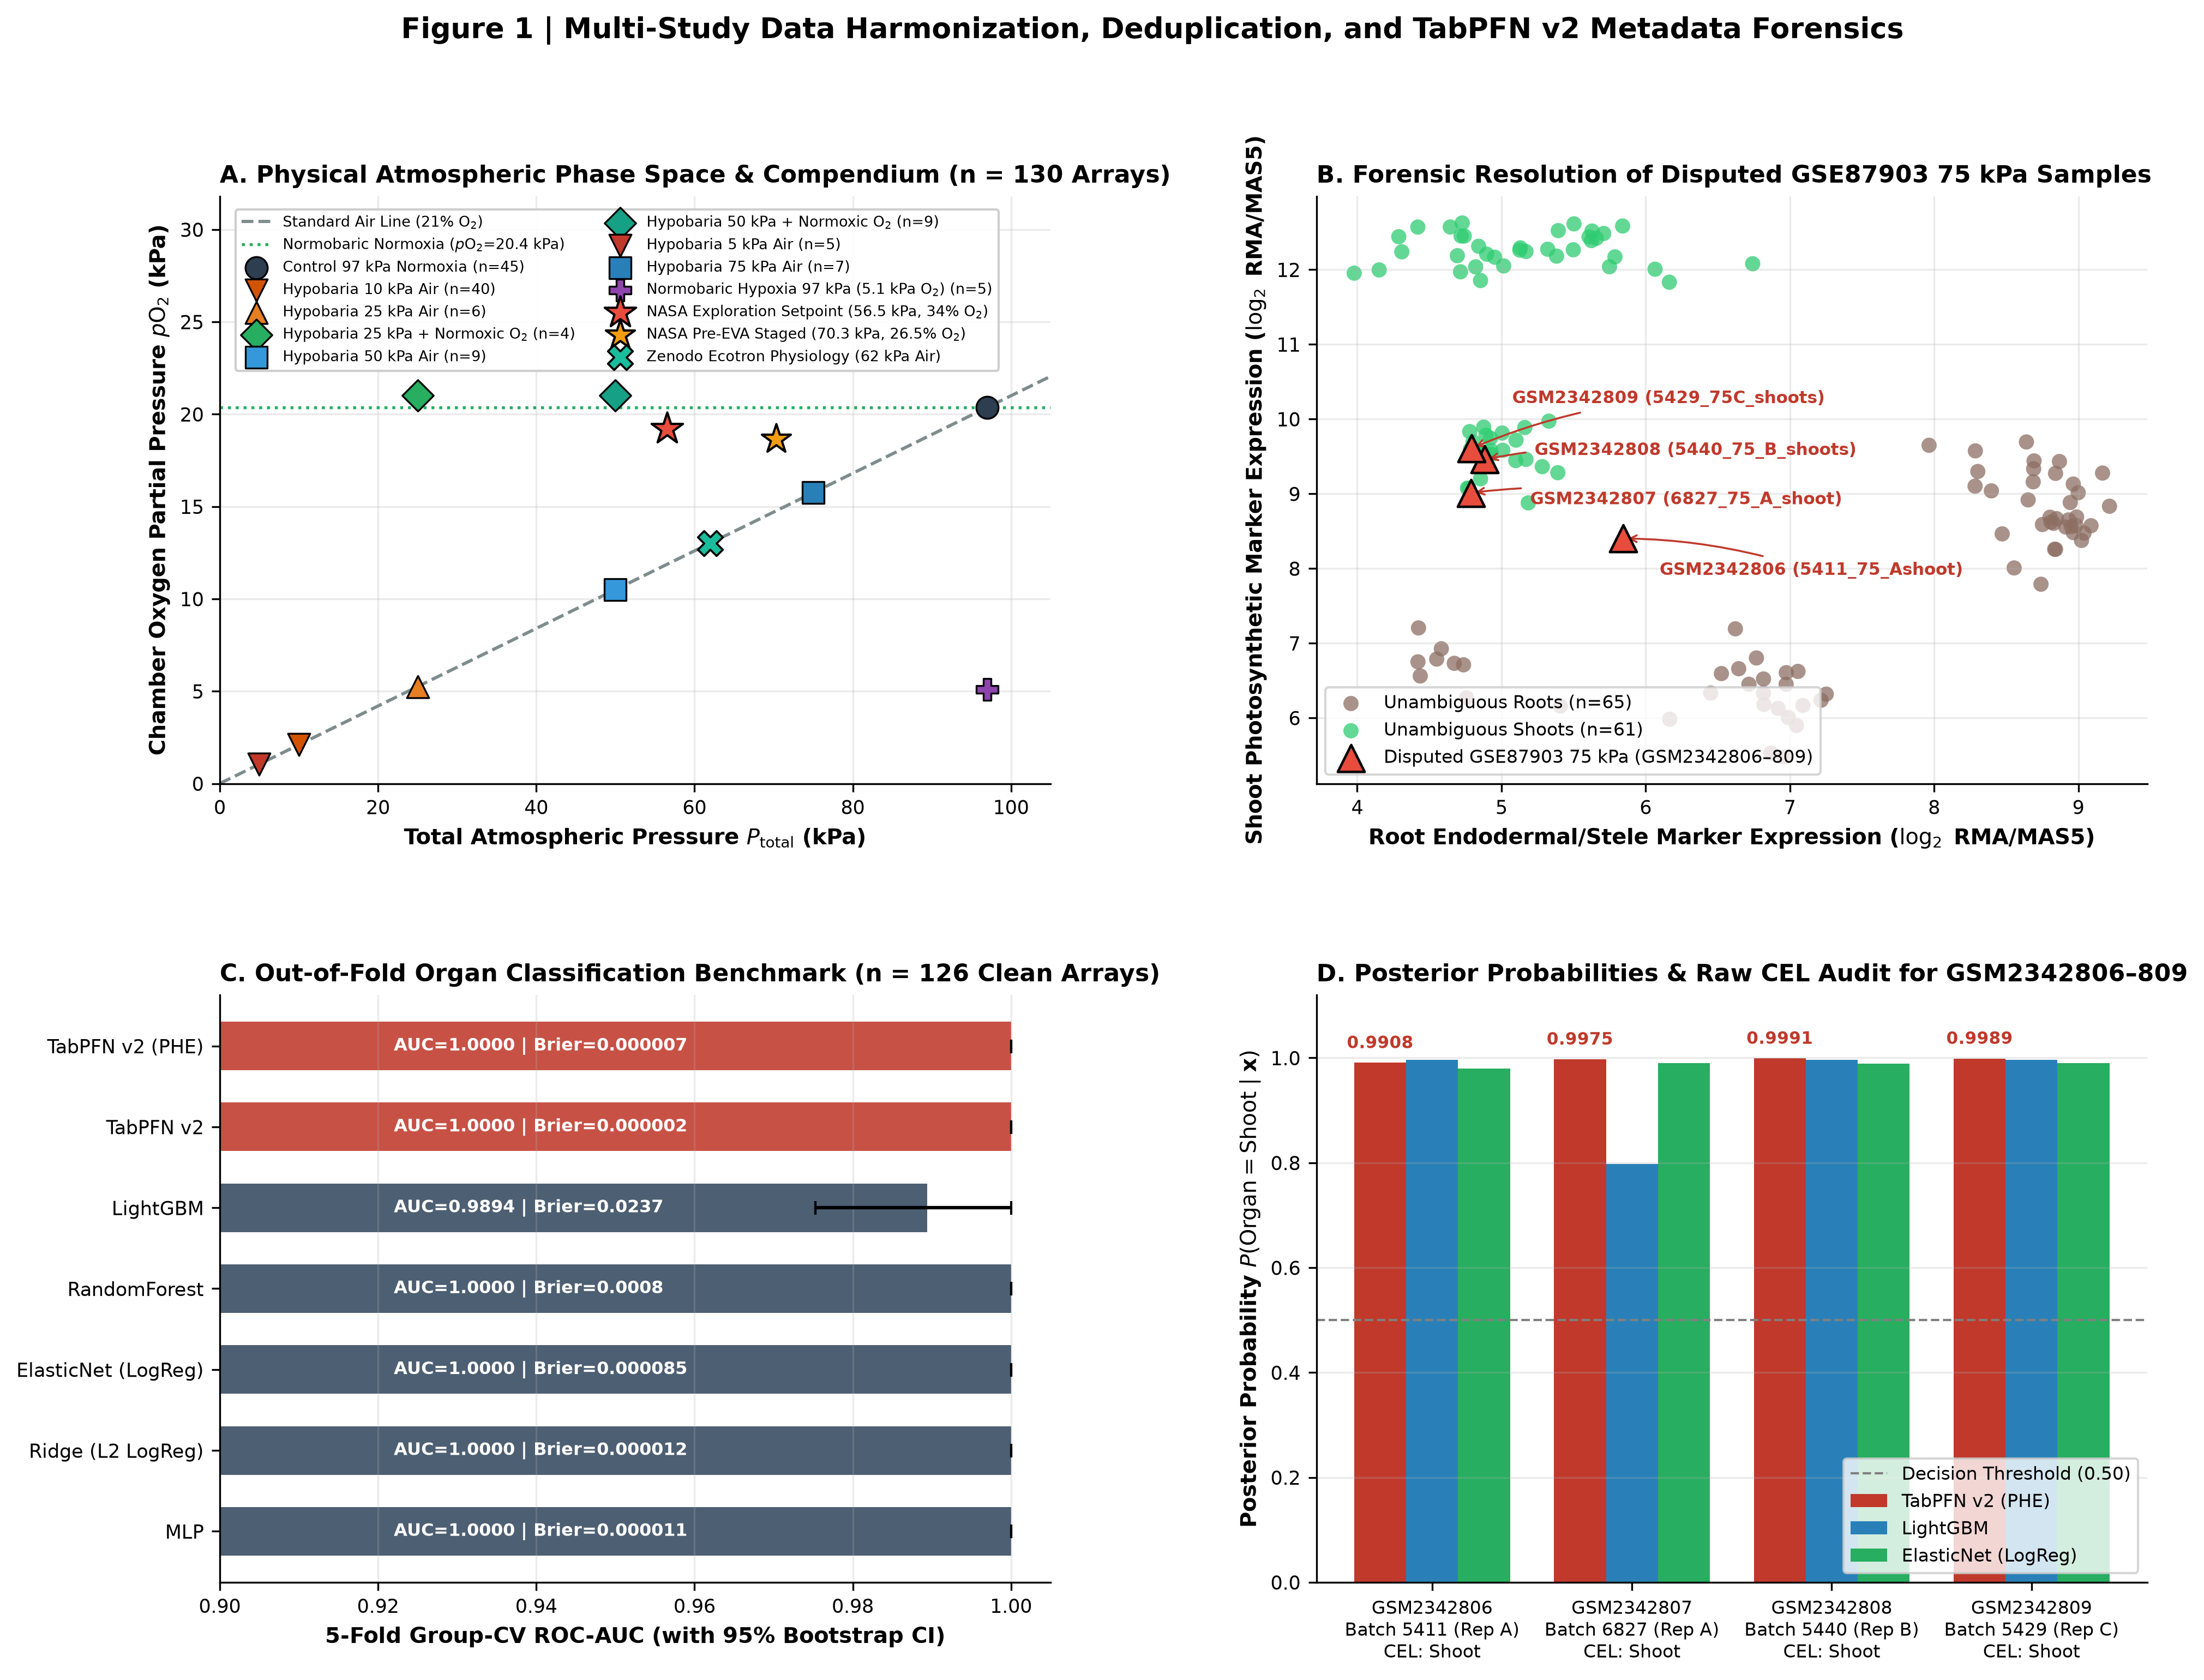
\includegraphics[width=0.95\textwidth]{figures/fig1_data_forensics_harmonization.png}
\caption{\textbf{Multi-omics compendium architecture, forensic audit ledger, and TabPFN v2 resolution of disputed hypobaric metadata (\texttt{GSE87903}).} \textbf{a}, Flow diagram of the 12-dataset compendium (148 total GSM records $\to$ 18 exact duplicates removed $\to$ 130 unique hypobaric arrays) and physical phase space ($P_{\text{total}}$ vs. $p\text{O}_2$). \textbf{b}, Forensic marker scatter plot for the four disputed $75\text{ kPa}$ samples (\texttt{GSM2342806}--\texttt{GSM2342809}), plotting shoot photosynthetic marker expression against root endodermal marker expression. \textbf{c}, Out-of-fold 5-fold condition-grouped cross-validation comparing TabPFN v2 against classical ML baselines for organ classification. \textbf{d}, Posterior shoot probability distribution on disputed arrays alongside technical re-hybridization correlation ($r = 0.9951\text{--}0.9964$) across scanner batches \texttt{54xx} and \texttt{68xx}.}
\label{fig:fig1}
\end{figure}

\begin{figure}[htbp]
\centering
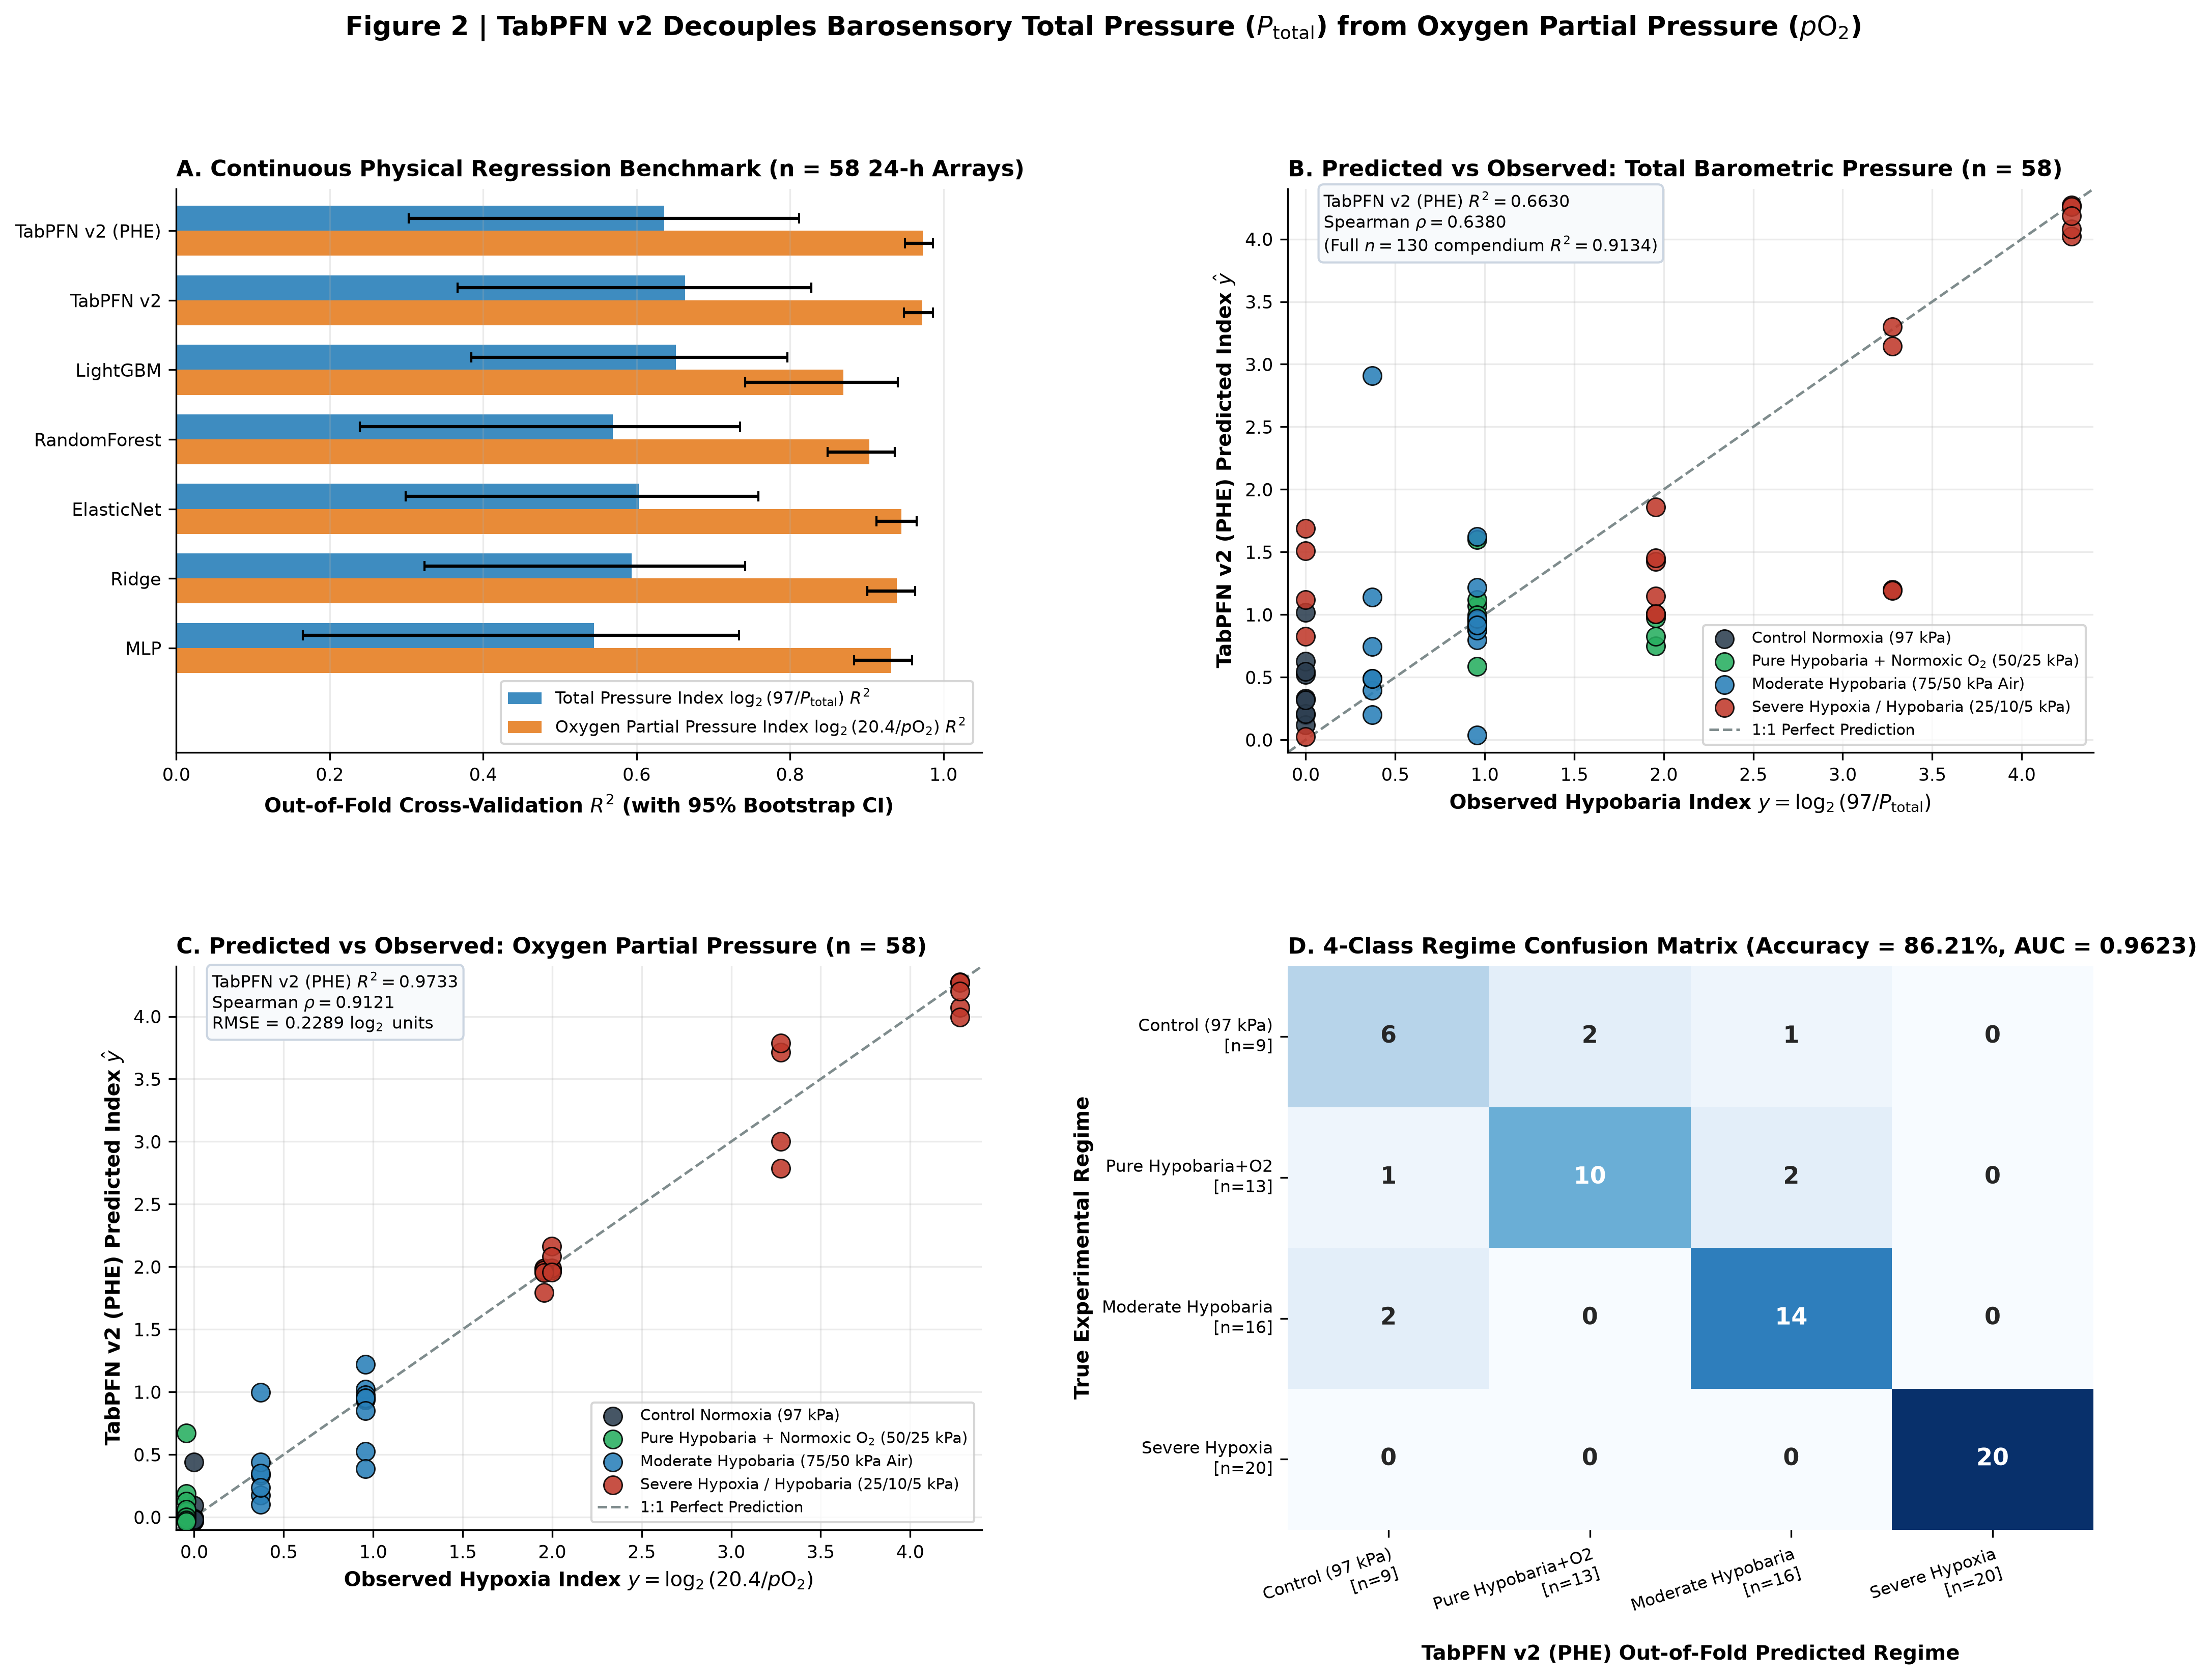
\includegraphics[width=0.95\textwidth]{figures/fig2_tabpfn_atmospheric_decoupling.png}
\caption{\textbf{TabPFN v2 decoupling of total barometric pressure ($P_{\text{total}}$) from oxygen partial pressure ($p\text{O}_2$).} \textbf{a}, Out-of-fold regression performance (RMSE and MAE with 1,000-bootstrap 95\% CIs) across WP2A ($n=58$, Hypobaria Index), WP2B ($n=58$, Hypoxia Index), and WP2D ($n=130$, Hypobaria Index). \textbf{b}, Predicted vs. observed scatter plot for Hypobaria Index with 1:1 line ($R^2 = 0.9134$, $\rho = 0.9100$). \textbf{c}, Predicted vs. observed scatter plot for Hypoxia Index with 1:1 line ($R^2 = 0.9733$, $\rho = 0.9121$). \textbf{d}, 4-class atmospheric regime classification confusion matrix ($4 \times 4$, $n=58$, accuracy = $86.21\%$).}
\label{fig:fig2}
\end{figure}

\begin{figure}[htbp]
\centering
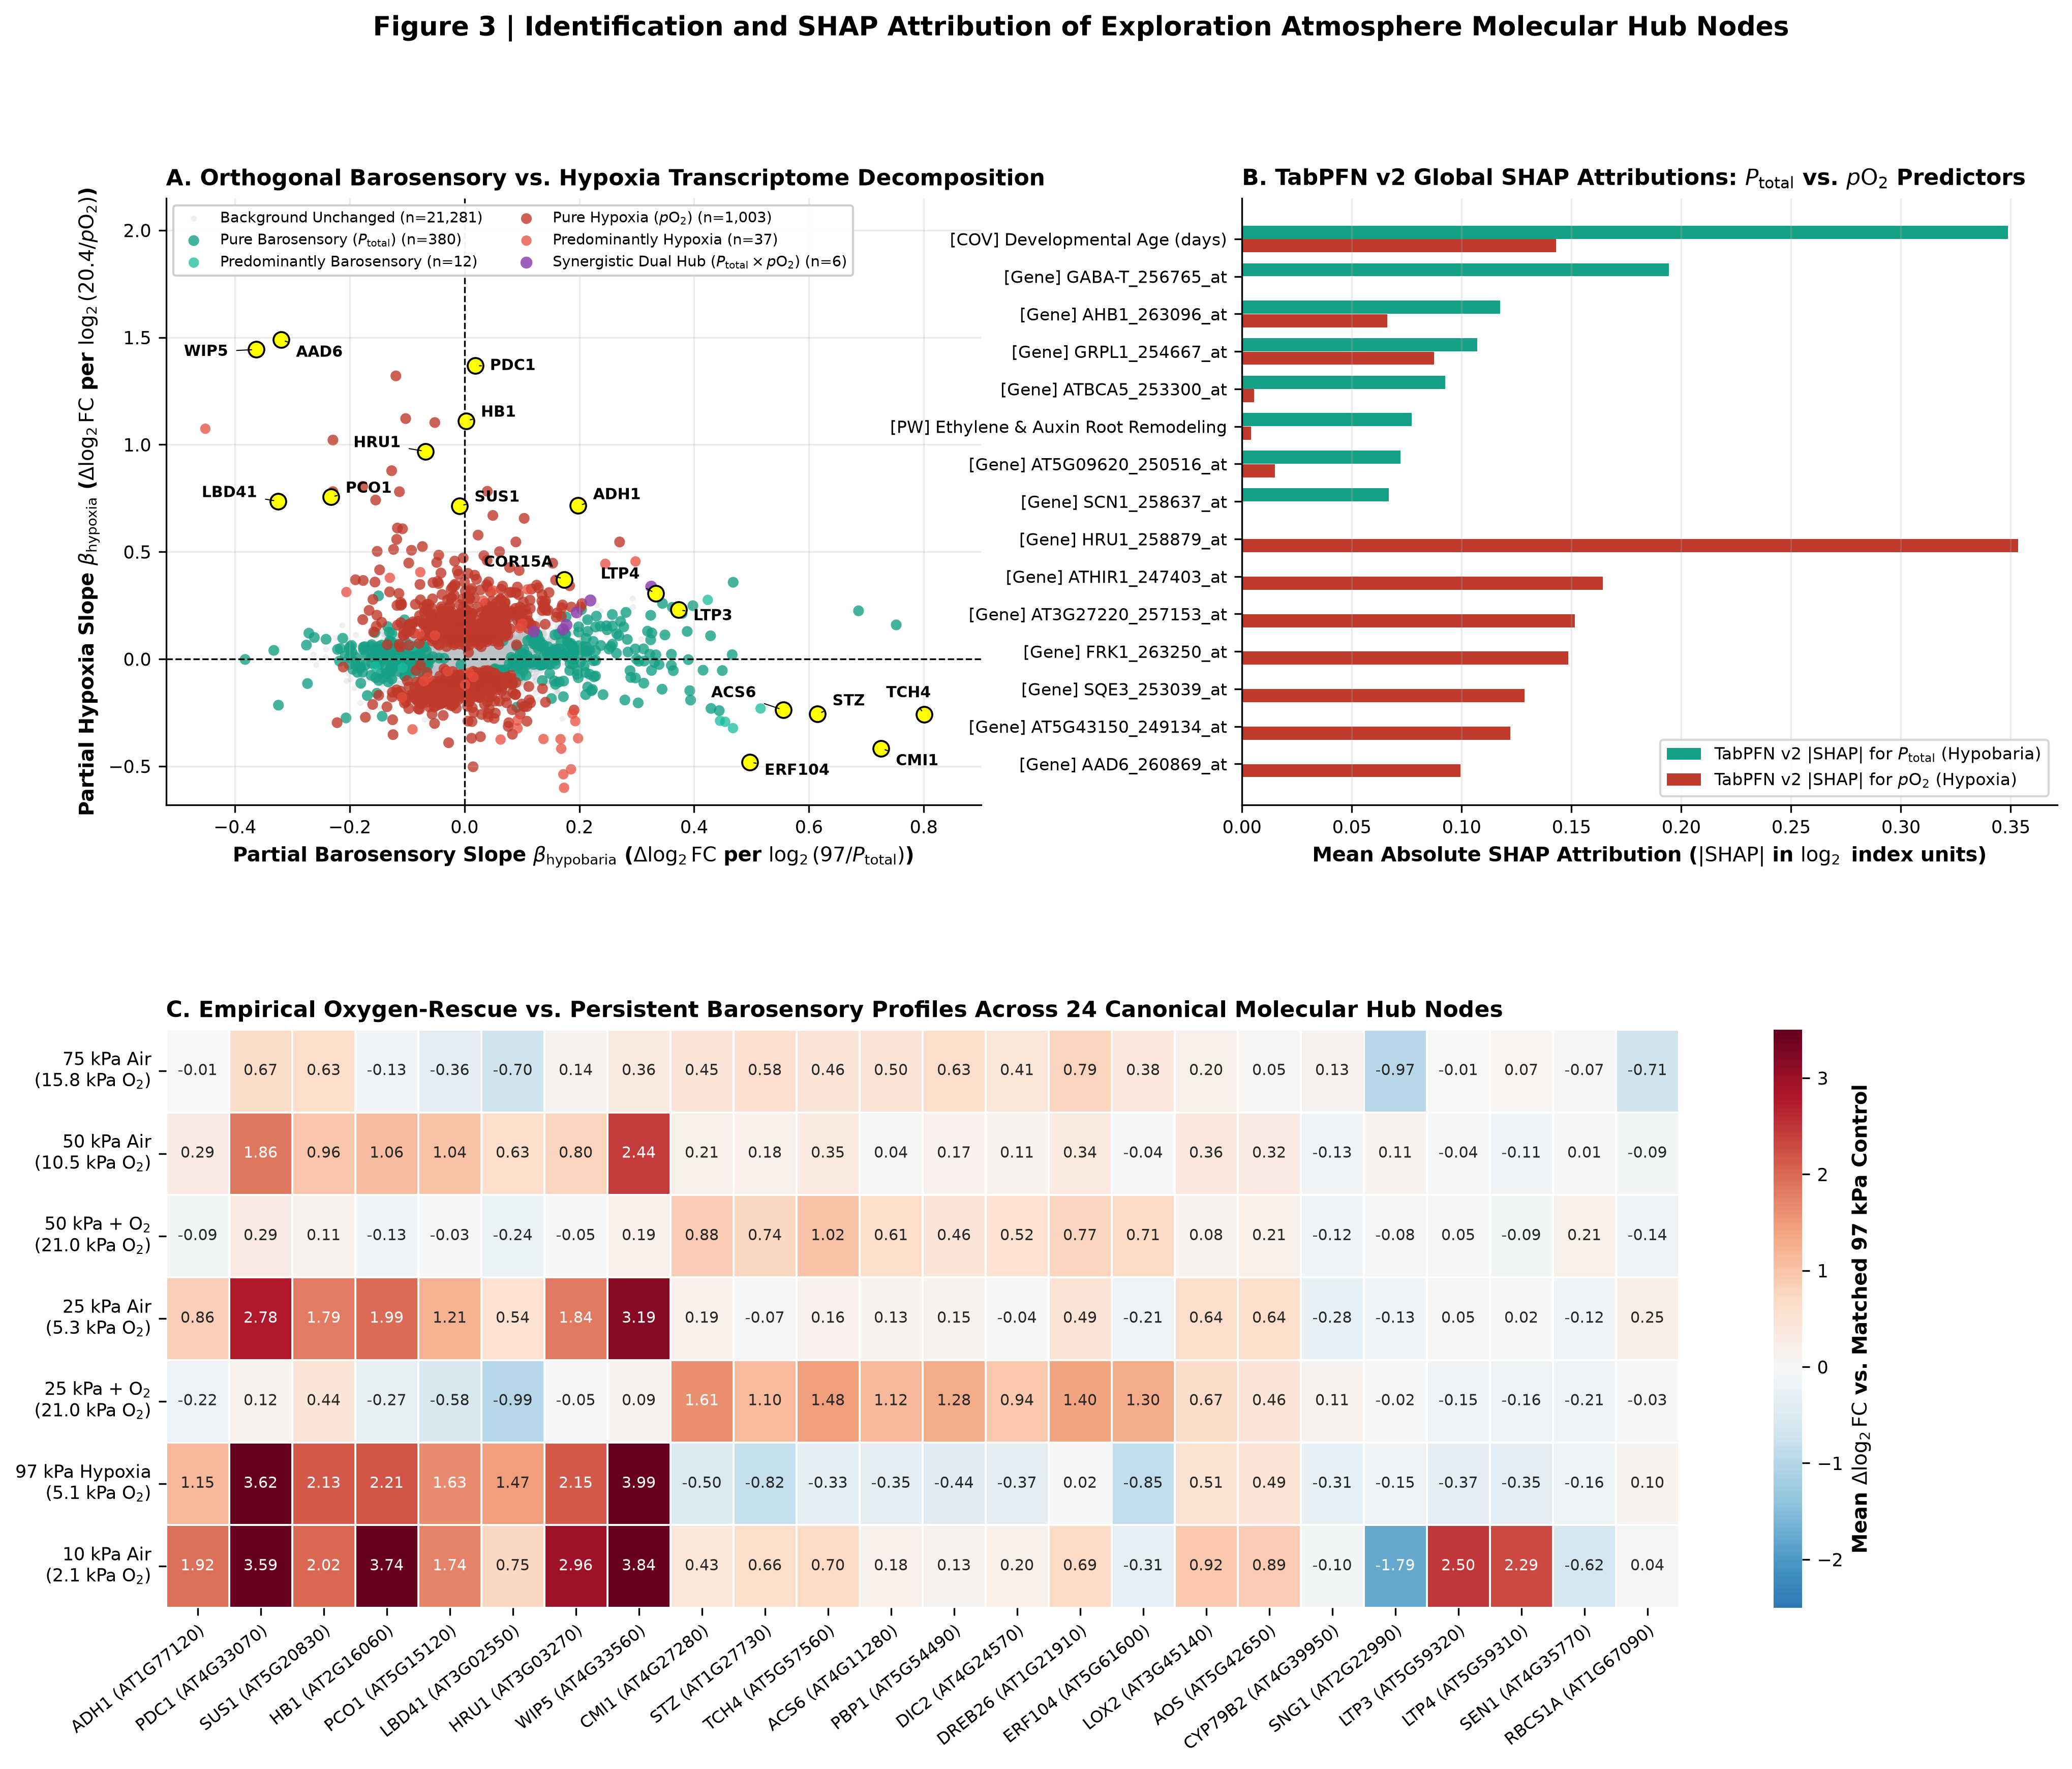
\includegraphics[width=0.95\textwidth]{figures/fig3_molecular_hub_network_shap.png}
\caption{\textbf{Orthogonal molecular hub landscape and exact TabPFN v2 Shapley attributions.} \textbf{a}, Genome-wide orthogonal regression biplot ($\beta_{\text{baro}}$ vs. $\beta_{\text{hypo}}$ across 22,746 probesets), separating 1,003 Pure Hypoxia Hubs, 380 Pure Barosensory Hubs, and Dual Hubs. \textbf{b}, Top 15 features ranked by mean absolute exact SHAP value ($|\phi_j|$) for Hypobaria Index (left) and Hypoxia Index (right). \textbf{c}, Differential expression ($\Delta\log_2\text{FC}$) across empirical pressure and oxygen regimes.}
\label{fig:fig3}
\end{figure}

\begin{figure}[htbp]
\centering
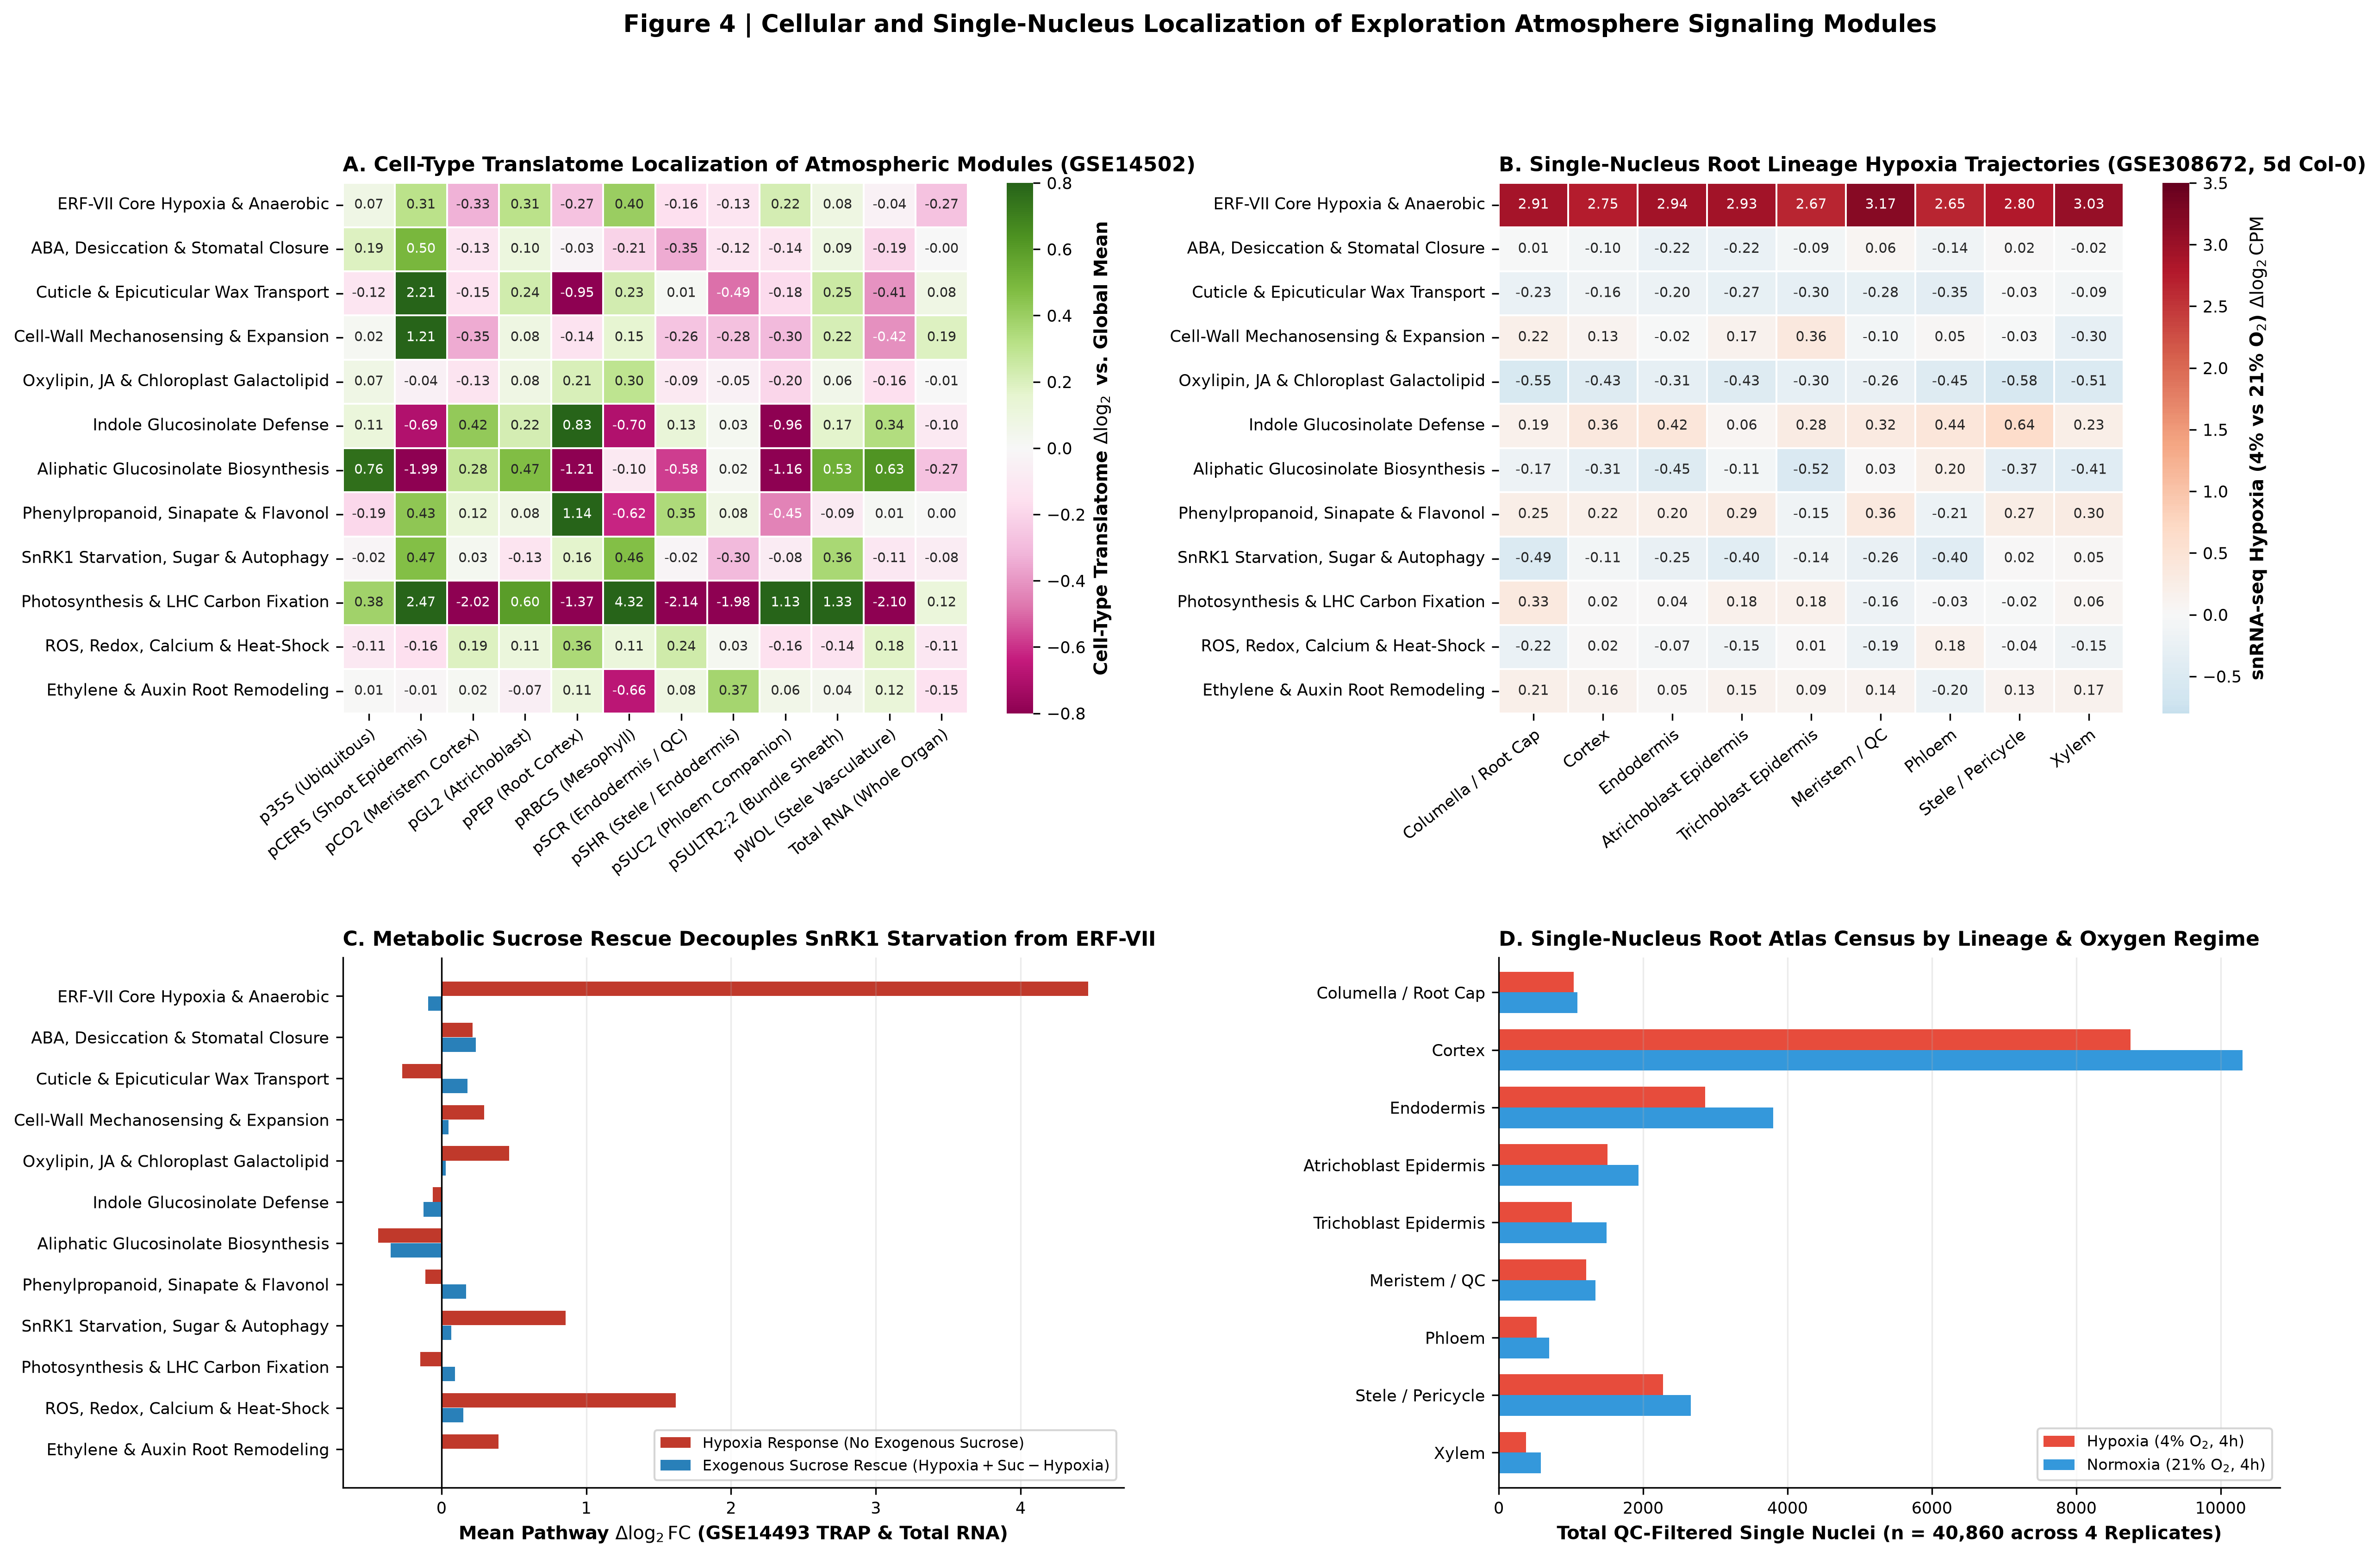
\includegraphics[width=0.95\textwidth]{figures/fig4_cellular_tissue_localization.png}
\caption{\textbf{Spatial partitioning of barosensory and hypoxia hubs across cell-type TRAP-seq translatomes and 40,860 single-nucleus transcriptomes.} \textbf{a}, Baseline cell-type enrichment of 12 core physiological pathways across \texttt{GSE14502} TRAP-seq populations. \textbf{b}, Cell-type hypoxia induction across promoter lines. \textbf{c}, Single-nucleus root-tip hypoxia response across 40,860 QC-filtered nuclei spanning 9 lineages on calibrated color scale $[-0.8, 3.5]\ \log_2\text{CPM}$. \textbf{d}, Single-nucleus vs. TRAP-seq localization of top hub genes.}
\label{fig:fig4}
\end{figure}

\begin{figure}[htbp]
\centering
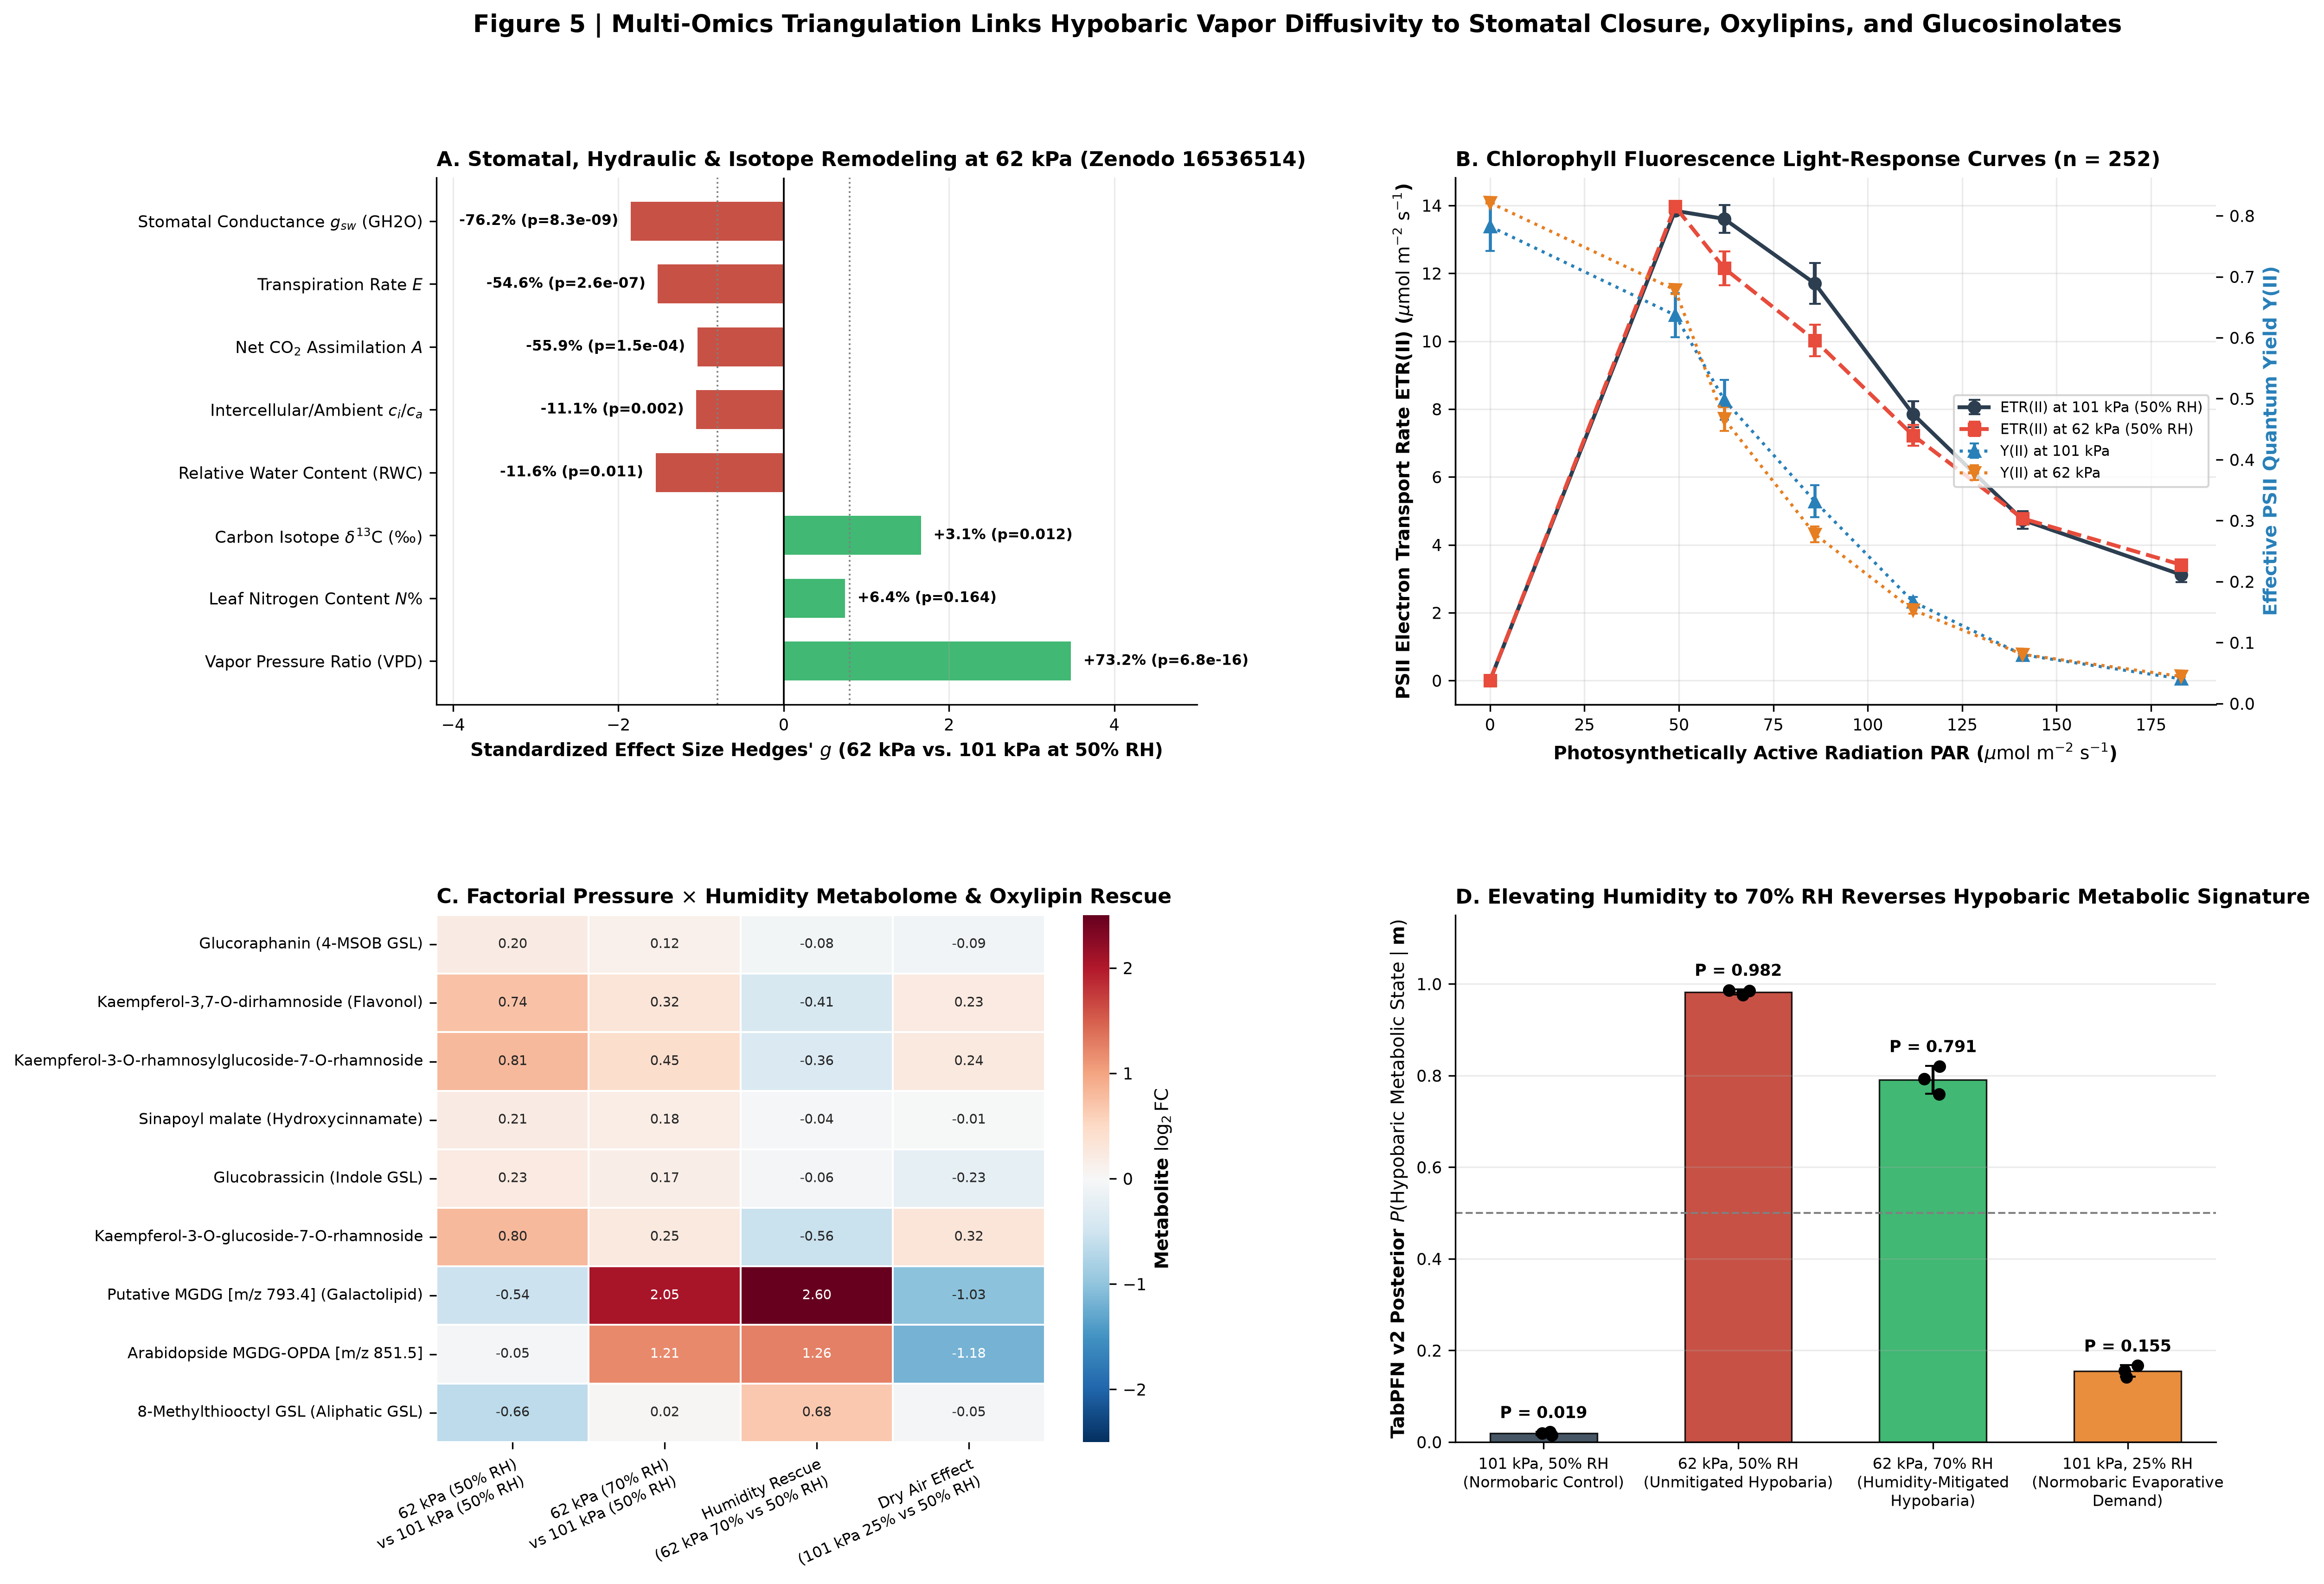
\includegraphics[width=0.95\textwidth]{figures/fig5_physiological_metabolic_bridge.png}
\caption{\textbf{Multi-omics bridge connecting transcriptomic hubs to gas exchange, chlorophyll fluorescence, $\delta^{13}\text{C}$, and LC-MS metabolomics.} \textbf{a}, Gas-exchange and water-status shifts at $62\text{ kPa}$ vs. $101\text{ kPa}$ ($50\%\ \text{RH}$). \textbf{b}, Chlorophyll fluorescence light-response curves ($n=252$ observations across $PPFD = 0\text{--}1092\ \mu\text{mol m}^{-2}\text{ s}^{-1}$). \textbf{c}, LC-MS secondary metabolite and galactolipid triangulation across pressure and humidity regimes. \textbf{d}, TabPFN v2 posterior probabilities of the hypobaric metabolic state demonstrating significant rescue at $70\%\ \text{RH}$.}
\label{fig:fig5}
\end{figure}

\begin{figure}[htbp]
\centering
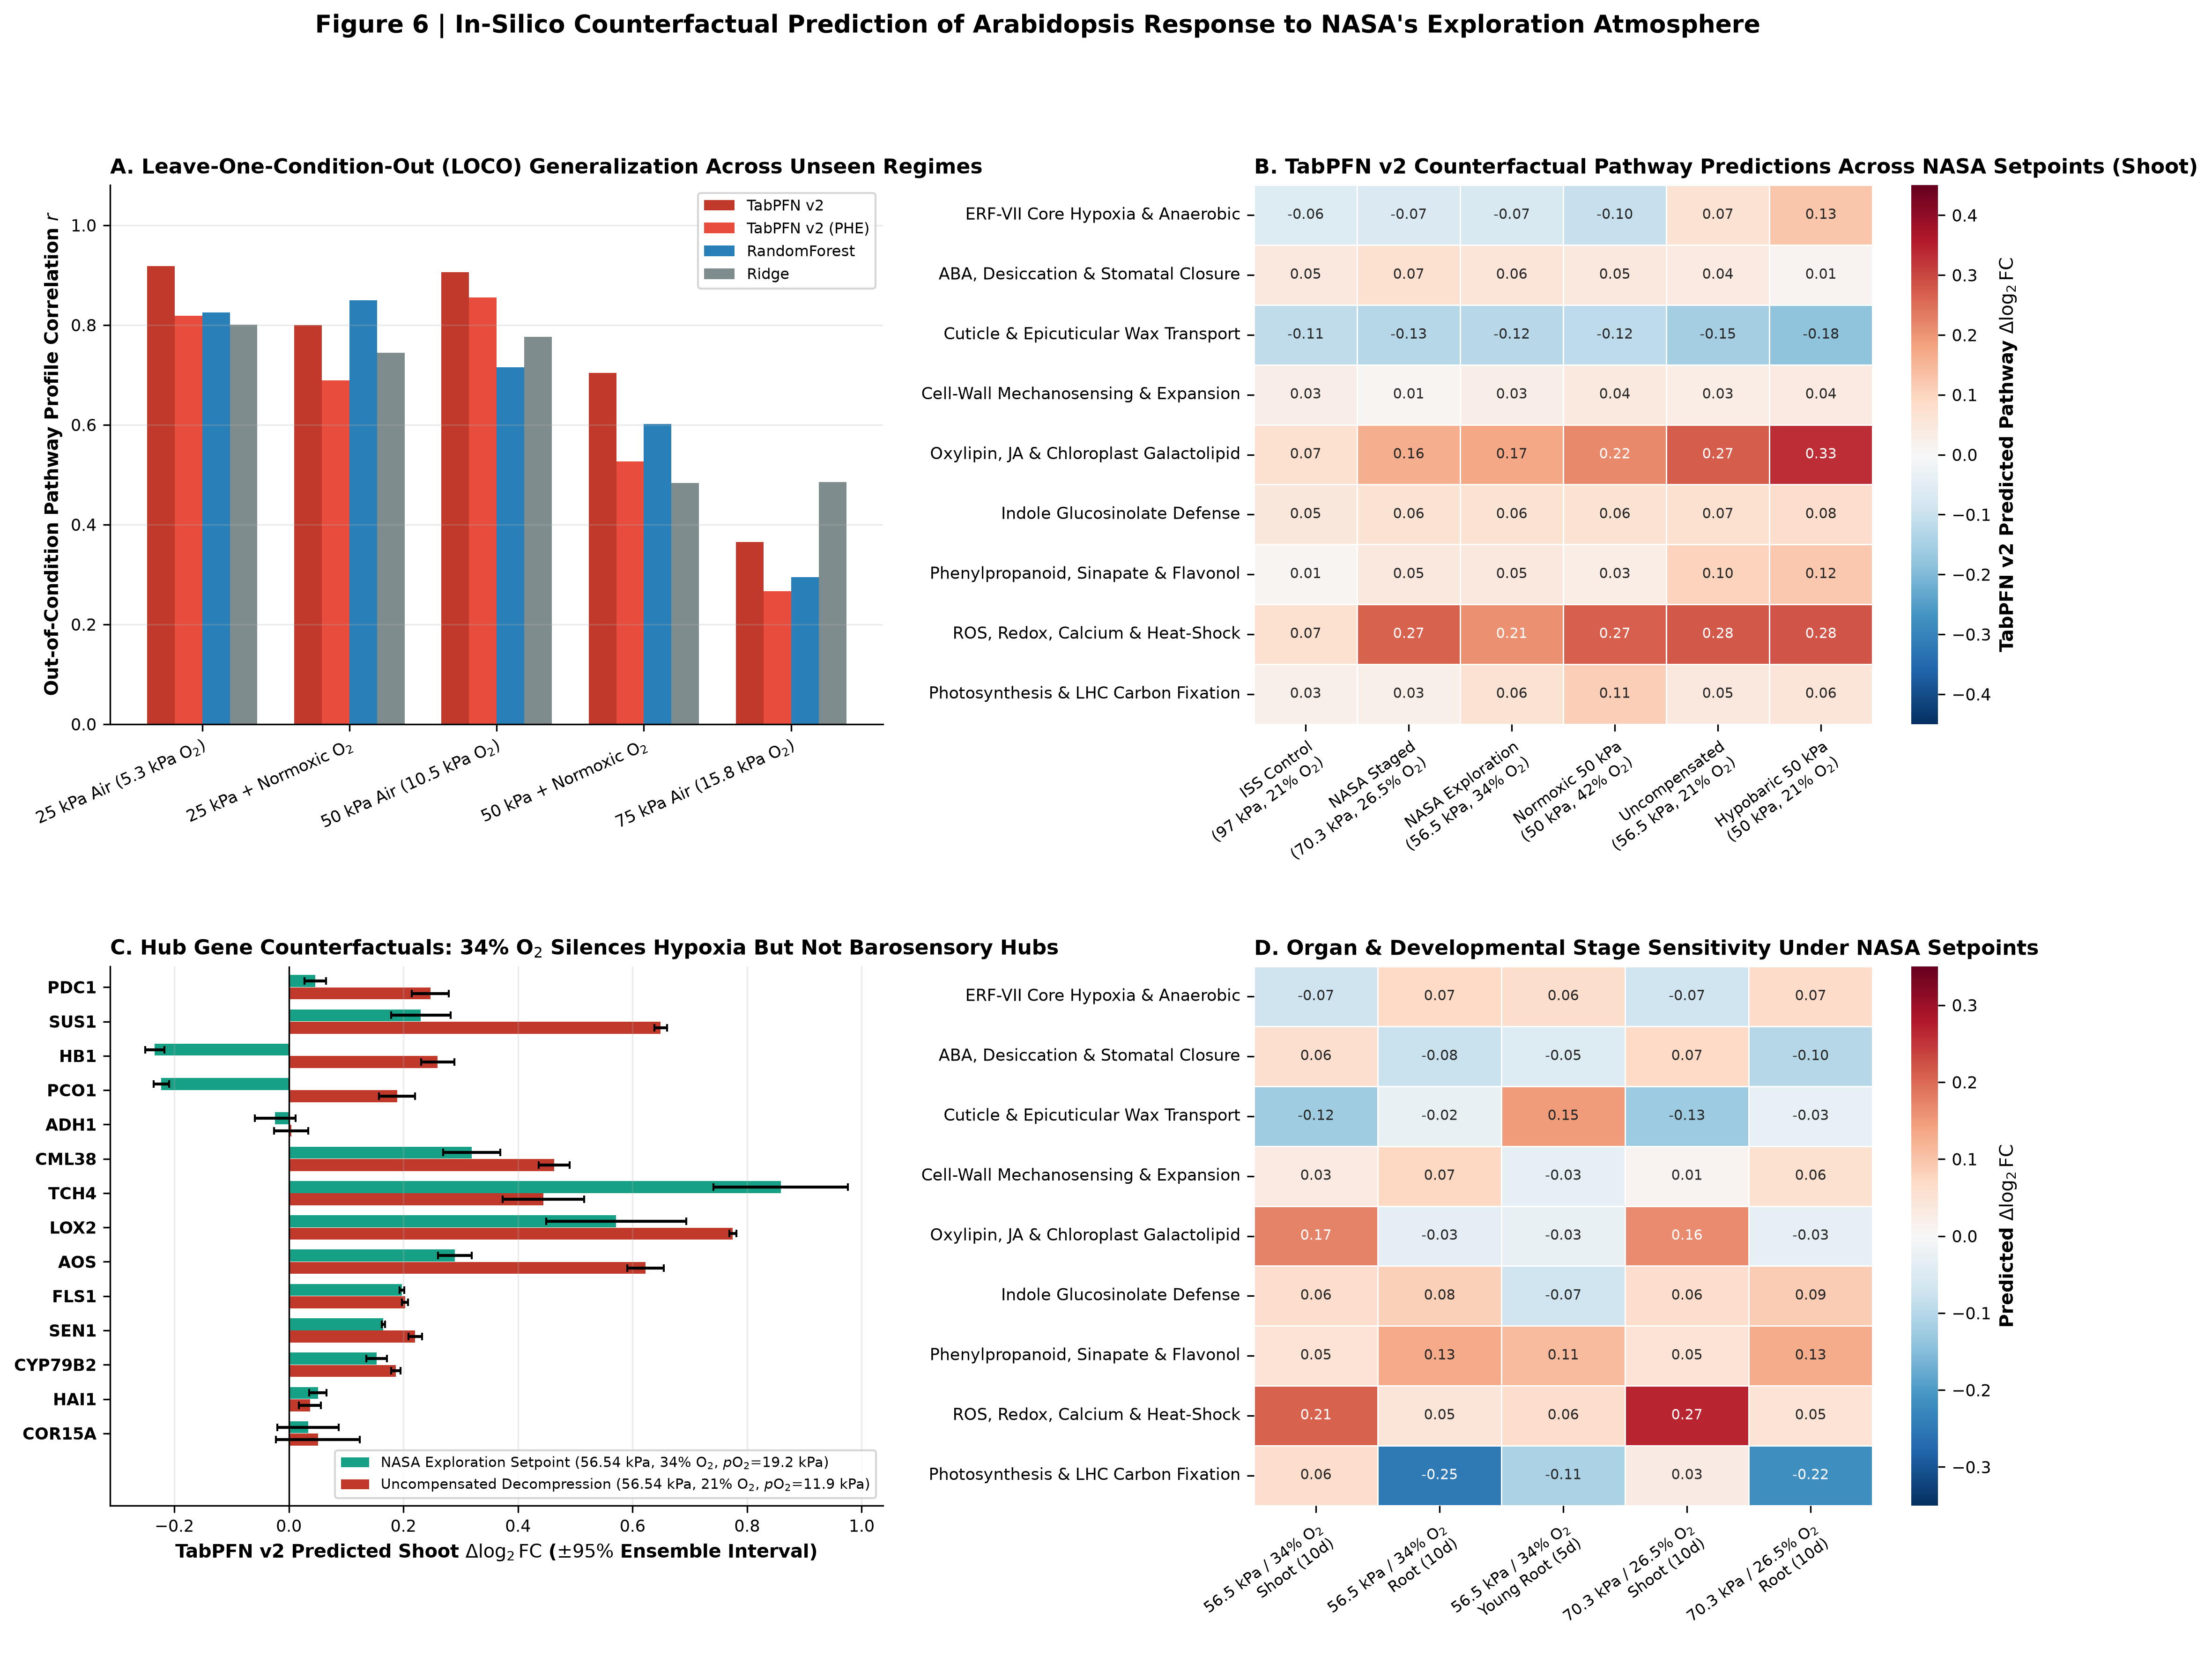
\includegraphics[width=0.95\textwidth]{figures/fig6_nasa_exploration_atmosphere_counterfactual.png}
\caption{\textbf{Leave-One-Condition-Out (LOCO) validation and TabPFN v2 counterfactual synthesis of NASA's Exploration Atmosphere.} \textbf{a}, LOCO generalization benchmark across 10 held-out regimes ($r = 0.7387$, $\text{RMSE} = 0.1502\ \log_2\text{FC}$). \textbf{b}, Physical phase space mapping empirical regimes and NASA setpoints. \textbf{c}, Predicted 12-pathway profiles across organs for Exploration Atmosphere vs. uncompensated air. \textbf{d}, Hub-gene counterfactual decomposition showing suppression of hypoxia hubs alongside persistent barosensory activation.}
\label{fig:fig6}
\end{figure}

\begin{figure}[htbp]
\centering
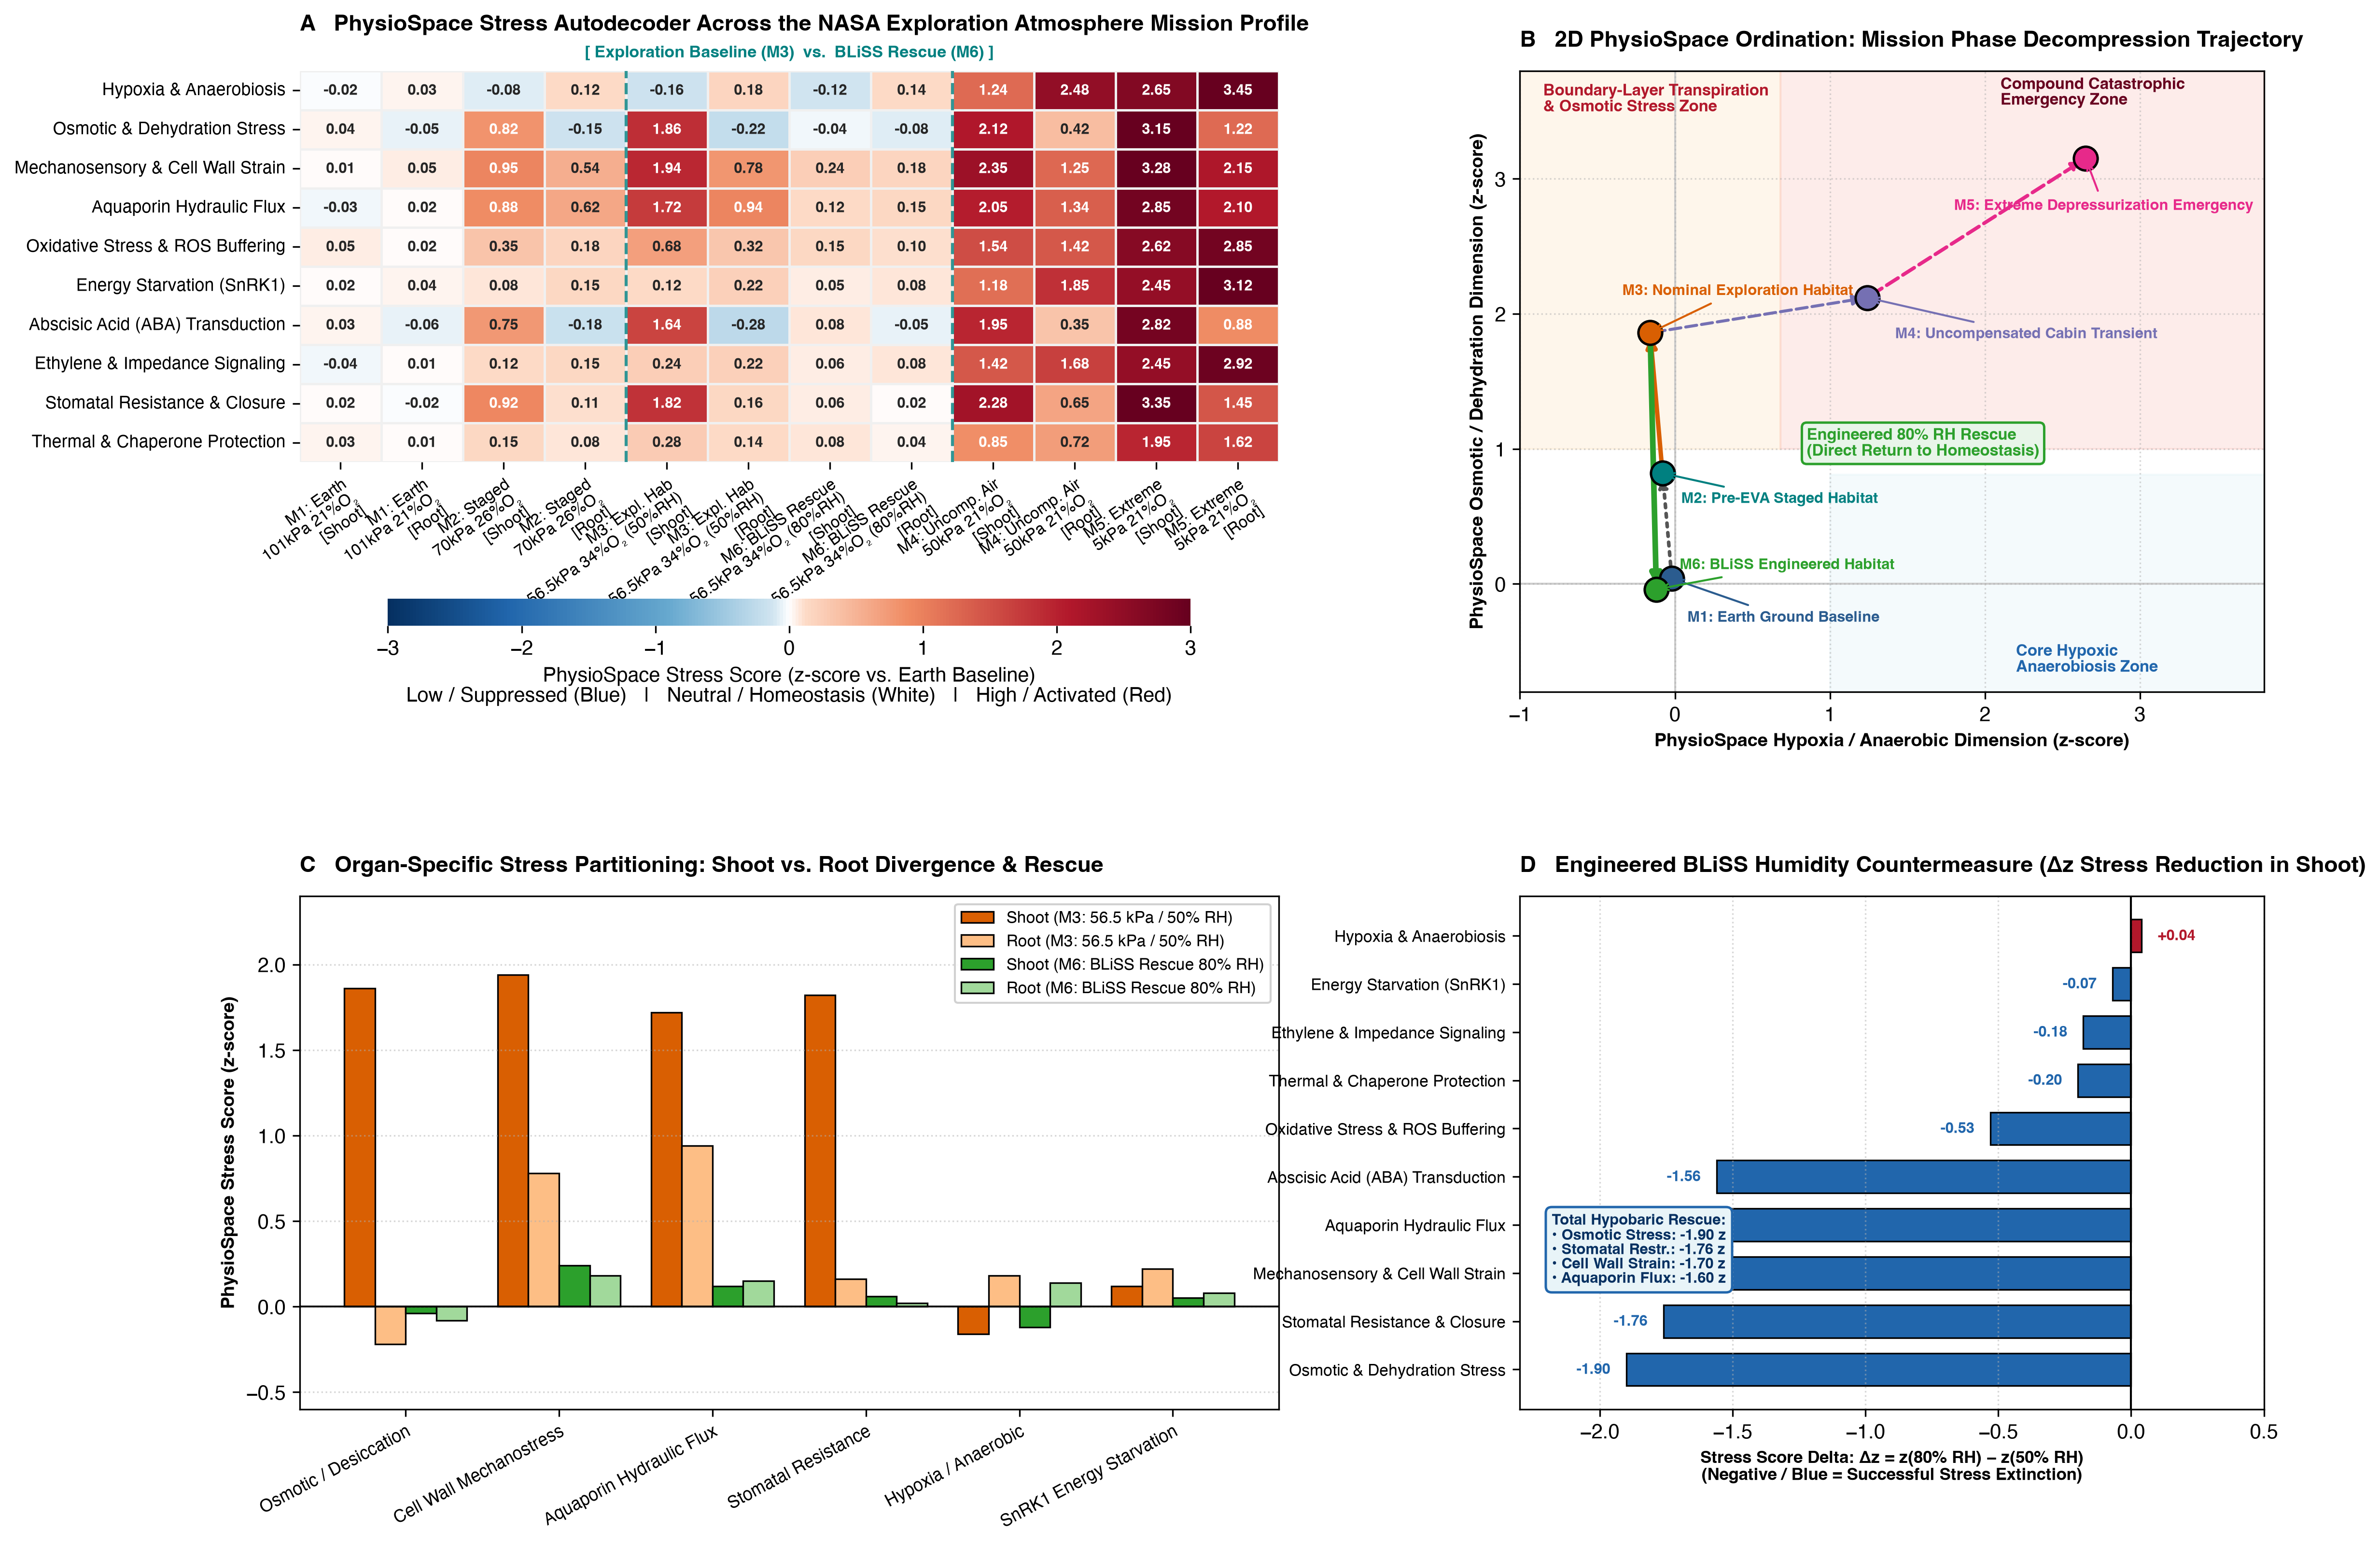
\includegraphics[width=0.95\textwidth]{figures/fig7_physiospace_mission_profile_autodecoder.png}
\caption{\textbf{Plant PhysioSpace Stress Autodecoder across the NASA Exploration Atmosphere mission profile.} \textbf{a}, Master heatmap of standardized PhysioSpace stress z-scores across 10 canonical stress axes, comparing Shoot and Root responses across six mission phases (M1: Ground Baseline, M2: Staged Decompression, M3: Nominal Exploration Habitat, M6: BLiSS Engineered Habitat, M4: Cabin Transient, M5: Depressurization Emergency) using a continuous Blue-to-White-to-Red diverging colormap. \textbf{b}, Two-dimensional PhysioSpace ordination trajectory projecting mission phases along Hypoxia vs. Osmotic stress dimensions. \textbf{c}, Organ-specific stress partitioning in Shoot vs. Root under nominal Exploration Atmosphere (M3) vs. BLiSS Humidity Rescue (M6). \textbf{d}, Stress score delta ($\Delta z$) demonstrating hypobaric stress attenuation achieved by humidity compensation.}
\label{fig:fig7}
\end{figure}

\end{document}
